\documentclass[12pt,letterpaperpaper,]{book}
\usepackage{lmodern}
\usepackage{amssymb,amsmath}
\usepackage{ifxetex,ifluatex}
\usepackage{fixltx2e} % provides \textsubscript
\ifnum 0\ifxetex 1\fi\ifluatex 1\fi=0 % if pdftex
  \usepackage[T1]{fontenc}
  \usepackage[utf8]{inputenc}
\else % if luatex or xelatex
  \ifxetex
    \usepackage{mathspec}
  \else
    \usepackage{fontspec}
  \fi
  \defaultfontfeatures{Ligatures=TeX,Scale=MatchLowercase}
    \setmonofont[Mapping=tex-ansi,Scale=0.8]{Source Code Pro}
\fi
% use upquote if available, for straight quotes in verbatim environments
\IfFileExists{upquote.sty}{\usepackage{upquote}}{}
% use microtype if available
\IfFileExists{microtype.sty}{%
\usepackage{microtype}
\UseMicrotypeSet[protrusion]{basicmath} % disable protrusion for tt fonts
}{}
\usepackage[margin=1.2in]{geometry}
\usepackage{hyperref}
\hypersetup{unicode=true,
            pdftitle={Prospectus},
            pdfauthor={Danton Noriega},
            pdfborder={0 0 0},
            breaklinks=true}
\urlstyle{same}  % don't use monospace font for urls
\usepackage{natbib}
\bibliographystyle{apalike}
\usepackage{longtable,booktabs}
\usepackage{graphicx,grffile}
\makeatletter
\def\maxwidth{\ifdim\Gin@nat@width>\linewidth\linewidth\else\Gin@nat@width\fi}
\def\maxheight{\ifdim\Gin@nat@height>\textheight\textheight\else\Gin@nat@height\fi}
\makeatother
% Scale images if necessary, so that they will not overflow the page
% margins by default, and it is still possible to overwrite the defaults
% using explicit options in \includegraphics[width, height, ...]{}
\setkeys{Gin}{width=\maxwidth,height=\maxheight,keepaspectratio}
\IfFileExists{parskip.sty}{%
\usepackage{parskip}
}{% else
\setlength{\parindent}{0pt}
\setlength{\parskip}{6pt plus 2pt minus 1pt}
}
\setlength{\emergencystretch}{3em}  % prevent overfull lines
\providecommand{\tightlist}{%
  \setlength{\itemsep}{0pt}\setlength{\parskip}{0pt}}
\setcounter{secnumdepth}{5}
% Redefines (sub)paragraphs to behave more like sections
\ifx\paragraph\undefined\else
\let\oldparagraph\paragraph
\renewcommand{\paragraph}[1]{\oldparagraph{#1}\mbox{}}
\fi
\ifx\subparagraph\undefined\else
\let\oldsubparagraph\subparagraph
\renewcommand{\subparagraph}[1]{\oldsubparagraph{#1}\mbox{}}
\fi
\usepackage{booktabs}
\usepackage{lscape}
\usepackage{longtable}
\usepackage{bm}
\usepackage{isomath}
\usepackage{setspace}
\usepackage[labelfont=bf, singlelinecheck=off, font={footnotesize}, textfont=sf]{caption}
% \doublespacing
\newcommand{\matr}[1]{\mathbf{#1}}
\newcommand{\blandscape}{\begin{landscape}}
\newcommand{\elandscape}{\end{landscape}}

%Ligatures=NoCommon very clutch for removing ligatures
\setromanfont[Mapping=tex-text, Ligatures=NoCommon]{Minion Pro}
\setsansfont[Mapping=tex-text, Ligatures=NoCommon]{Source Sans Pro}
\setmonofont[Mapping=tex-text,Scale=0.8]{Source Code Pro}

\usepackage{framed,color}
\definecolor{shadecolor}{RGB}{248,248,248}

\renewcommand{\textfraction}{0.05}
\renewcommand{\topfraction}{0.8}
\renewcommand{\bottomfraction}{0.8}
\renewcommand{\floatpagefraction}{0.75}

% \renewenvironment{quote}{\begin{VF}}{\end{VF}}
\let\oldhref\href
\renewcommand{\href}[2]{#2\footnote{\url{#1}}}

\ifxetex
  \usepackage{letltxmacro}
  \setlength{\XeTeXLinkMargin}{1pt}
  \LetLtxMacro\SavedIncludeGraphics\includegraphics
  \def\includegraphics#1#{% #1 catches optional stuff (star/opt. arg.)
    \IncludeGraphicsAux{#1}%
  }%
  \newcommand*{\IncludeGraphicsAux}[2]{%
    \XeTeXLinkBox{%
      \SavedIncludeGraphics#1{#2}%
    }%
  }%
\fi

\makeatletter
\newenvironment{kframe}{%
\medskip{}
\setlength{\fboxsep}{.8em}
 \def\at@end@of@kframe{}%
 \ifinner\ifhmode%
  \def\at@end@of@kframe{\end{minipage}}%
  \begin{minipage}{\columnwidth}%
 \fi\fi%
 \def\FrameCommand##1{\hskip\@totalleftmargin \hskip-\fboxsep
 \colorbox{shadecolor}{##1}\hskip-\fboxsep
     % There is no \\@totalrightmargin, so:
     \hskip-\linewidth \hskip-\@totalleftmargin \hskip\columnwidth}%
 \MakeFramed {\advance\hsize-\width
   \@totalleftmargin\z@ \linewidth\hsize
   \@setminipage}}%
 {\par\unskip\endMakeFramed%
 \at@end@of@kframe}
\makeatother

\newenvironment{rmdblock}[1]
  {
  \begin{itemize}
  \renewcommand{\labelitemi}{
    \raisebox{-.7\height}[0pt][0pt]{
      {\setkeys{Gin}{width=3em,keepaspectratio}\includegraphics{images/#1}}
    }
  }
  \setlength{\fboxsep}{1em}
  \begin{kframe}
  \item
  }
  {
  \end{kframe}
  \end{itemize}
  }
\newenvironment{rmdnote}
  {\begin{rmdblock}{note}}
  {\end{rmdblock}}
\newenvironment{rmdcaution}
  {\begin{rmdblock}{caution}}
  {\end{rmdblock}}
\newenvironment{rmdimportant}
  {\begin{rmdblock}{important}}
  {\end{rmdblock}}
\newenvironment{rmdtip}
  {\begin{rmdblock}{tip}}
  {\end{rmdblock}}
\newenvironment{rmdwarning}
  {\begin{rmdblock}{warning}}
  {\end{rmdblock}}

\usepackage{makeidx}
\makeindex

\urlstyle{tt}

\usepackage{amsthm}
\makeatletter
\def\thm@space@setup{%
  \thm@preskip=8pt plus 2pt minus 4pt
  \thm@postskip=\thm@preskip
}
\makeatother

\title{Prospectus}
\author{Danton Noriega}
\date{March 16, 2017}

\begin{document}
\maketitle

\setlength{\abovedisplayskip}{-5pt}
\setlength{\abovedisplayshortskip}{-5pt}
\mainmatter

{
\setcounter{tocdepth}{2}
\tableofcontents
}
\chapter*{Dissertation Overview}\label{dissertation-overview}
\addcontentsline{toc}{chapter}{Dissertation Overview}

The broader goal of my dissertation is to explore existing policies
aimed at improving access to, the coverage of, and the efficacy of,
government assistance programs. I will do so in three studies. The first
measures the impact of a financial incentive that may or may not
increase access to fresh produce for SNAP participants. The second
investigates if a low-cost, universal nurse home-visiting program can,
as a secondary effect, help eligible families receive assistance sooner
and/or more frequently. The third aims to continue building the case
that in-kind transfer programs, while critical to families coping with
poverty, remain insufficient, leaving families to reach out for extra
support from friends, family, or emergency services.

\section*{Chapter Summaries}\label{chapter-summaries}
\addcontentsline{toc}{section}{Chapter Summaries}

Chapter 1 is an evaluation of the effectiveness of the Double Up Food
Bucks program. I define ``effectiveness'' as the change in total sales
and volume of produce sold within 17 grocery stores that implement
Double Up (treatment group), compared to the control group of 15 stores
where Double Up was not implemented. In anticipation of data challenges,
I recommend models frameworks for measuring the size of the effect.

Improving health and food equity of SNAP participants is the broader
policy concern. The mechanism is a financial incentive---Double Up Food
Bucks---designed to increase fruit and vegetable consumption. A
comparison will be made with another financial incentive program called
the \emph{Healthy Incentives Pilot} (HIP). I will argue how and why an
evaluation of the Double Up program is an important addition to the
current literature.

Chapter 2 exploits the random assignment of the Durham Connects program
to measure its long term impact on social service applications. Durham
Connects (DC) provided free in-home nursing visits to recent mothers in
Durham County. DC was implemented as an RCT between July 2009 to
December 2010. The design treats DC as an information treatment. The DC
information treatment (e.g.~a nurse contact to ask questions and provide
assistance) is expected to lower the learning and barrier costs of
low-income families with children when applying for social services.

Chapter 3 aims to build on the work of
\citet{schenck-fontaine_use_2016}. Through surveys,
\citet{schenck-fontaine_use_2016} examine how families coping with
poverty and economic instability supplement their SNAP benefits with
informal and formal resources. In my paper, I hope to build a better
understanding of how and when families use emergency resources provided
by local-governments and charities. I aim to do this by analyzing food
pantry donations data and administrative records of emergency assistance
applications.

\chapter{An Evaluation of the Double Up Food Bucks
program}\label{chapter-1}

\section*{Motivation}\label{motivation}
\addcontentsline{toc}{section}{Motivation}

\textbf{Research Question}

\begin{quote}
How effective is the DUFB financial incentive at increasing the fresh
fruits and vegetables purchased by SNAP shoppers within a grocery store
environment?
\end{quote}

\textbf{Hypothesis 1}: I expect a slight increase (1 - 2\%) in SNAP EBT
expenditures on fruits and vegetables (FVs) during the months the DUFB
incentive is active in the experimental stores (Aug - Dec). I expect the
effect will fade over time. I expect no significant differences in fruit
and vegetable expenditures during the months the incentive is not in
effect (Jan - July).

The DUFB incentive is automatic. (covered in more detail in the
\protect\hyperlink{data-1}{Data Section}). By default, all SNAP shoppers
at a DUFB store are technically ``participating''. I think of SNAP
shoppers as being ``passive'' or ``active'' participants. ``Active
participation'' would characterize shoppers responding to the DUFB
incentive; ``passive participation'' would characterize shoppers who
continue to shop as usual, despite automatically redeeming points.

I know from prior implementations of the program that participation
rates in DUFB-like incentive programs can be low. In this case, I expect
SNAP shoppers to consist of mostly ``passive'' participants. Combined
with the fact that SNAP dollars account for less than 5\% of all
spending in these stores, I don't think there is a large pool of SNAP
participants to draw from. As a result, the ``active'' participants, who
respond to the incentive and buy more fruits and vegetables, will
consist of a small fraction of total FV spending. I expect that
comparing all FV purchases between treatment and control stores would
fail to find any distributional differences. Instead, to measure the
impact of the incentive, I will have to focus on, and compare, purchases
made by the targeted group (SNAP households) in both types of stores.

I don't know if the corporate office, which selected and implemented the
DUFB incentive, properly communicated or advertised the DUFB program to
store management/staff and customers. This likely resulted in low
awareness of the DUFB program amongst store staff and shoppers. Low
participation may correlate highly with low awareness. Meaning, low
participation may not be a failure of DUFB program as an incentive
mechanism, but a failure of corporate advertising and ``buy-in''. I must
be clear that this is merely a hunch. I don't think there is a large
profit motive behind implementing this program for the retailer. I think
this was an opportunity to pretend to be doing some good and to have
something which reflects a positive corporate image. A survey of store
staff and of some customers to test this hunch would be great.

\textbf{Hypothesis 2}: If measurable, I expect spending increases to
occur within the first 3 weeks of each calendar month, when most SNAP
benefits are distributed and consumed. I also expect spending with SNAP
benefits during the 4th calendar week of each month for all stores to be
similar, regardless of DUFB participation. That is, if I observe any
differences in SNAP benefit spending, it will be during the 1st, 2nd,
and 3rd week of each calendar month, but not the 4th.

Prior research found that SNAP shoppers spend their benefits soon after
receiving them, generally in one large shopping trip
\citep{wiig_art_2009, damon_first_2013}. The grocery stores are located
in a state where benefits are disbursed every odd day of the month
between the 3rd and 21st, spanning the first 3 weeks of each month.
Therefore, by the 4th week, total unspent dollars across all SNAP
households will be at a minimum. Since the DUFB incentive is triggered
by the use of SNAP benefits, many SNAP shoppers will be unable, or
unwilling, to make use of DUFB having already spent most, if not all, of
their benefits for the month.

I expect that, were I to remove the 4th week of each month from all
stores, the DUFB effect size will increase. I do not expect to see
shoppers behave in strategic saving behavior of DUFB points (which is
difficult given the automatic accrual and redemption system) nor do I
think FV spending will increase much without the presence of the
incentive. More importantly, since I cannot link purchases to
individuals (more on this later), it will be impossible to identify
transactions made by SNAP shoppers anytime they do not use their EBT
cards.

\section*{Introduction}\label{intro-1}
\addcontentsline{toc}{section}{Introduction}

Chronic conditions like obesity, heart disease, and other metabolic risk
factors (stroke, type II diabetes, etc.) cost the US health care system
between 200 to 400 billion dollars annually
\citep{cawley_medical_2012, chatterjee_checkup_2014}. More importantly,
these diseases account for hundreds of thousands of deaths each year.
Heart disease alone is the leading cause of death for all persons in the
US, with stroke fifth and diabetes seventh
\citep{national_center_for_health_statistics_health_2015}. Diet is
closely linked to these conditions, particularly obesity and
cardiovascular disease. Strong evidence shows that a diet high in (1)
vegetables, fruits, nuts, unsaturated oils, fish, and poultry, but low
in (2) red and processed meat and sugar-sweetened foods and drinks,
helps lower body weight, blood pressure, and the risk of cardiovascular
disease
\citep{mente_systematic_2009, nutrition_evidence_library_series_2014}.
Improving the diet of Americans has therefore become an increasing
priority for the United States, especially for families in the
Supplemental Nutrition Assistance (SNAP) program.

SNAP is a federal aid program administered by the Food and Nutrition
Service (FNS), an agency of the U.S. Department of Agriculture (USDA).
At 74 billion dollars in FY2015 with 45.8 million participants, it is
the largest food assistance program in the United States
\citep{usda_fns_supplemental_2016}. To be eligible for SNAP, a household
must be sufficiently budget constrained that hunger is considered likely
without assistance. Eligibility is a function of countable resources,
vehicle ownership and value, household size, gross or net monthly
income, household composition, and meeting certain work
requirements.\footnote{For more details, visit
  \url{http://www.fns.usda.gov/snap/eligibility}} Some eligibility
requirements vary by state, but in general, a family with dependents,
less than \$2000 in countable resources, where the adults work at least
part-time earning a gross (net) monthly income at or below 130\% (100\%)
of the federal poverty line, is eligible to receive SNAP benefits. Aside
from a few restrictions---no alcohol, tobacco, non-food items,
ready-to-eat meals, or hot foods---households can use SNAP benefits to
buy any foods for at-home consumption. Unfortunately, the purchasing
patterns of the average SNAP household are not conducive to a healthy
diet.

Research on the dietary patterns of households receiving SNAP benefits
has found that they are significantly \emph{less} likely to meet USDA
dietary guidelines than the average US household and much \emph{more}
likely to consume unhealthy foods
\citep{andreyeva_dietary_2015, nguyen_supplemental_2015, wolfson_fruit_2015}.
A smaller set of research has found that SNAP households, at best,
consume the same amount of unhealthy foods (e.g.~sugar-sweetened
beverages, baked goods, snacks, candy, etc) compared to SNAP-ineligible
households \citep{todd_caloric_2014, hoynes_snap_2015}. In other words,
SNAP households consume foods that are less healthy or about the same as
SNAP-ineligible households. This is a concerning result given that most
US households, regardless of income, already purchase and consume far
too much meat and foods rich in sugars and fats, and far too few fruits,
vegetables and whole grains
\citep{usda_scientific_2015, frazao_high_1999}. The purpose of SNAP,
however, is to keep struggling families from going hungry, not to ensure
they consume the best possible diet. SNAP is designed to act like cash,
helping families access more food than they could otherwise do so
without assistance \citep{hoynes_snap_2015}. It is therefore not a
failing of the SNAP program if benefits are used to purchase unhealthy
foods.

The SNAP program could be changed such that it could continue satisfying
its role as an anti-hunger program while simultaneously encouraging
healthier purchases. \citet{blumenthal_strategies_2014} and
\citet{leung_qualitative_2013} both surveyed a field of stakeholders and
policy experts in the SNAP program about what they would do to improve
the dietary quality of purchases. In both studies, restricting the
purchase of unhealthy foods (e.g.~sugar-sweetened beverages) and
promoting healthy purchases through monetary incentives were the two
most popular improvements (i.e.~ranked the highest or most often
suggested).\footnote{It should be mentioned that there were other, less
  popular recommendations, such as modifying how SNAP benefits are
  distributed and improving nutrition education. For more details, see
  \citet{blumenthal_strategies_2014} and \citet{leung_qualitative_2013}.}

One common suggestion is to restrict the SNAP program to the same set of
eligible foods as the Special Supplemental Nutrition Program for Woman,
Infants, and Children (WIC) \citep{dinour_food_2007}. The WIC program
provides food vouchers that limit households to a select group of food
products. These food products are specifically selected to ensure women
and their children receive nutritious, healthy foods. In other words,
the WIC program, by design, places restrictions on food choices by
defining a list of \emph{eligible} items, as opposed to the SNAP
program, which defines a list of \emph{ineligible} items. Another
common, and simpler, suggestion is to expand the existing list of
ineligible items (e.g.~alcohol) with products that are unambiguously
lacking in nutrition and easy to identify, like soda or candy. New York
City, for example, attempted to ban sugar-sweetened beverages, and the
state of Maine attempted to restrict sodas, candy, and any other taxable
food items \citep{gundersen_snap_2015}. The USDA overturned both
restrictions.

Problems exists with ``improving'' the SNAP program by implementing even
greater purchasing restrictions. First, there is no reason to believe
that such a restriction would work. The restriction assumes that, under
WIC-like requirements, households will substitute healthy foods for
unhealthy foods when using SNAP benefits. What would most likely happen
is that households would shift to purchasing unhealthy foods with cash.
Second, such restrictions would likely lead to a drop in SNAP
participation \citep{gundersen_snap_2015}. Restricting choice is a
paternalistic policy that would further stigmatize SNAP participation.
It would give the impression that SNAP beneficiaries are assumed to have
worse diets and that they cannot be trusted to make healthy food
purchases. Participation would also drop due to increased transaction
costs of purchasing items with SNAP. Not all stores would clearly mark
which items were SNAP eligible nor should participants be expected to
remember. The result would be longer, more frustrating shopping trips.
Lastly, it is important to remember that for many SNAP recipients,
freedom of choice is what makes the SNAP program popular and easy to use
\citep{edin_snap_2013}.

The most popular ``improvement'' was providing a monetary incentive to
SNAP participants for purchasing healthy foods
\citep{blumenthal_strategies_2014, leung_qualitative_2013}. Monetary (or
financial) incentives, in this context, tend to be a rebate or voucher
awarded to SNAP households for using their benefits to buy certain
healthful foods, generally mineral-rich and nutrient-dense fruits and
vegetables (i.e.~leafy greens but not white potatoes). These monetary
incentives for buying ``targeted'' fruits and vegetables (aka TFVs) are
exclusive to SNAP participants. Much like a grocery stores loyalty card
or a student ID card, retailers can ``discriminate on price'' (aka
``target the incentive'') using SNAP Electronic Benefit Transfer (EBT)
cards to identifying eligible participants. Monetary incentives in the
food retail environment are popular for two main reason. First, the
framing of the ``improvement'' is positive. Instead of ``punishing''
SNAP participants through paternal restriction or disincentives (not
covered), monetary incentives reward participants for healthy shopping
behavior \citep{gundersen_snap_2015}. Retailers also prefer the positive
framing of monetary incentives. For the moment, monetary incentives
programs for SNAP participants are not wide spread. Taking up an
incentive program, assuming the cost of implementation isn't too
expensive, creates an opportunity for retailers to differentiate
themselves from their competitors \citep{hartmann_corporate_2011}. The
second reason is a strong theoretical framework established by
neoclassical economics supporting incentives as an effective mechanism
for changing human behavior. In practice, however, incentives have had
mixed results, but there is building evidence that incentives may work
in the food retail space.

How, why, and to what effect incentives may encourage SNAP participants
to buy more targeted fruits and vegetables is the motivating question
behind this paper.

\subsection*{Financial Incentives to Encourage Healthy Food
Purchases}\label{financial-incentives-to-encourage-healthy-food-purchases}
\addcontentsline{toc}{subsection}{Financial Incentives to Encourage
Healthy Food Purchases}

Encouraging healthy behavior through financial incentives has a long
history. Results are mixed. For example, financial incentives have been
shown to help individuals commit to regular exercise, improve dieting,
increase weight loss, and to quit smoking, but the intended effect of
the financial incentives were often short-term (see
\citet{gneezy_when_2011} and \citet{cawley_economy_2015} for an
overview). \citet{gneezy_when_2011} also explain, through a review of
the literature, that depending on the context and design, incentives can
backfire, producing an effect known as ``crowd out''. Crowd out occurs
when an incentive displaces the intrinsic reward of a behavior
(originally defined for ``prosocial'' behavior, like volunteering or
giving blood; see \citet{benabou_incentives_2006}). The behavior then
becomes dependent on the extrinsic reward. As a result, having shifted
from being intrinsically rewarding to extrinsically rewarding, the
positive behavior continues only as long as the monetary incentive is
provided. More significantly, the intrinsic reward of the behavior does
not return once it has been ``crowded out''. Therefore, the long-term
effect of a monetary incentive can be negative, despite showing positive
effects in the short-term. That said, incentives can produce successful
long-term results if they are instead used as a mechanism to build good
habits. This requires that the incentives be salient and produce
immediate feedback without neglecting behavioral findings such as loss
aversion and mental accounting \citep{john_financial_2011}.

Given the research on incentives, it is reasonable to assume that a
monetary incentive for SNAP participants to purchase healthy foods, like
fruits and vegetables, may fail or even backfire. Should the act of
purchasing healthy foods be intrinsically rewarding to SNAP shoppers,
introducing an incentive may produce a ``crowd out'' effect. However,
recent field experiments find that incentives can establish healthy food
choice as a habit, possibly overriding any crowd out. Daily incentives
encourage children to make healthier food choices in school lunchrooms,
who in turn develop positive, long-term food habits
\citep{loewenstein_habit_2016, list_behavioralist_2015, belot_incentives_2014}.
Outside of the school lunchroom environment,
\citet{list_incentives_2015} found that similar habit formation is
possible with incentives in a more traditional food retail environment.
In their experiment, \citet{list_incentives_2015} provided an incentive
to 222 shoppers (\$1) to use their rewards cards, but then randomly
assigned each participant to the control group to one of three
interventions: \emph{information}, \emph{incentive}, or
\emph{combination}. The \emph{information} treatment was a flier with
tips on how to prepare fruit and vegetable dishes as well as the health
benefits of eating more fruits and veggies. The \emph{incentive} was an
additional dollar for every 5 cups of targeted fruits and vegetables
(TFVs) purchased. The \emph{combination} treatment group included both.
The intervention lasted for 5 months but each group continued to be
observed for roughly 6 weeks months after. The \emph{information}
intervention had no effect, but the \emph{incentive} and
\emph{combination} interventions on average doubled their purchase of
fruits and vegetables in comparison to the control group. Most
promisingly, the gap persisted with minimal shrinkage for 6 weeks
following the end of the intervention. However, there was no follow up
after the 6-week post-intervention period. It is therefore possible the
gap closed over multiple months (as opposed to multiple weeks).

The design, food environment, and target of the incentive in each of
these experiments is important. First, the incentive in these
experiments is designed to be salient and immediate. In the school
lunchroom experiments, the children are aware of the incentive and
receive the reward (e.g.~a small token) immediately after selecting the
healthy food item. Likewise, the shoppers received their additional one
dollar reward for every 5 cups of TFVs at checkout. One distinction
between the designs is frequency. The children are exposed to the
incentive every school day in the lunchroom experiments. The shoppers,
on the other hand, were exposed as frequently or as infrequently as they
chose. This distinction is important, as the latter better reflects the
experience of shoppers using the SNAP benefits. Second, the food
environment is important because it determines what choices are
available. The children have a finite set of options in the school
lunchroom and they also have no outside option (besides not eating
lunch). The children optimize on a relatively small set of choices and,
for the duration of the intervention, the incentive always existed. Food
retail environments are drastically different. There are numerous
competing food choices and generally other outside options.\footnote{It
  should be noted that this is not always the case. In
  \citet{list_incentives_2015}, for example, the store that was selected
  for the experiment was one of the few places local shoppers could find
  fresh produce. The store itself was located in one of Chicago's
  poorest neighborhoods.} It is substantially more difficult for the
shopper to optimize over such a large set of choices. Last, and most
obviously, one set of studies targets children, the other adults. A
priori, we would expect a monetary incentive to affect children
differently than adults. But the fact that habit formation through
incentives appears possible for both target groups is promising.

Research where SNAP participants are the target group is nascent. The
USDA's Food and Nutrition Services (FNS) ran the first large scale
randomized control trial investigating the impact of a financial
incentive for targeted fruits and vegetables in 2011. The experiment was
called the Healthy Incentives Pilot (HIP). HIP is the major precursor to
every incentive program currently being funding by the USDA. It also
provides the data for the few papers recently published on incentives
for SNAP participants.

\subsection*{The Healthy Incentives
Pilot}\label{the-healthy-incentives-pilot}
\addcontentsline{toc}{subsection}{The Healthy Incentives Pilot}

A brief overview of the Healthy Incentives Pilot is necessary to provide
context to, and contrast with, more recent financial incentive programs.

The UDSA's Food and Nutrition Services designed the Healthy Incentives
Pilot. The pilot was funded by the Food, Conservation, and Energy Act of
2008 to test whether financial incentives would increase consumption of
targeted fruits and vegetables (TFVs). SNAP participants were the target
group.

HIP was designed as a large scale randomized control trial (RCT). FNS
partnered with the Massachusetts Department of Transitional Assistance
to implement HIP. The pilot lasted from early 2011 to the end of 2012.
The population included all 55,095 SNAP participants in Hampden County,
MA. Hampden County is the poorest county in Massachusetts and has the
highest rates of obesity and other diet-related chronic illness
(e.g.~type 2 diabetes).

Of the 55,095 SNAP participants, 7,500 were randomly assigned to the
treatment group. The remainder fell into the control group. The
treatment was a 30 cent (or 30\%) rebate on every dollar spent on TFVs.
The rebate was capped at \$60 per month. To receive the rebate, selected
SNAP participants had to use their EBT cards at participating retailers.
The rebate, which was returned to their EBT account, could then be used
on any food item. That is, the rebate could only be earned buying TFVs,
but could be redeemed buying any SNAP eligible food item. Most HIP
participants spent about \$12 a month on TFVs, earning an average of
\$3.65 per month in rebates---drastically lower than the \$60 per month
rebate cap.

The evaluation was conducted using 24-hour dietary recall surveys. A
total of 5,000 participants were selected to be surveyed, even split
between treatment and control (2,500 HIP, 2,500 non-HIP). The first
survey was conducted prior to the start of the pilot. This established a
baseline. The second survey occurred 4 to 6 months in to the pilot and
the third survey occurred 9 to 11 months in. (The variation, e.g.~4 to 6
months, was due to the treatment being implemented in 3 waves of 2500.)

The evaluation found that the 30\% rebate lead to about a 26\% increase
in consumption of TFVs. This was equivalent to about 0.24 cups of TFVs.
Roughly 60\% of the increase was due to increased vegetable consumption
and 40\% due to increased fruit consumption. The effect, in absolute
terms (0.24 cups), seems small. But a \(0.87\) price elasticity,
relative to other results in the literature, is quite high---\(0.7\) and
\(0.48\), on average, for fruits and vegetables, respectively
\citep{andreyeva_impact_2010}.

Despite some limitations and technical problems---underreporting on the
24-hour recall survey and system glitches early in the pilot (see pages
60 and 208-210 of \citet{bartlett_evaluation_2014})---HIP was considered
to be an overall success
\citep{klerman_short-run_2014, olsho_financial_2016}. It implemented on
of the largest, most complex RCTs to isolate how incentives can increase
household consumption of TFVs. It also provided a feasible model for
nationwide expansion (assuming cost reductions due to economies of
scale; see \citet{an_nationwide_2015}).

HIP also provides a framework for understanding how a financial
incentive, expanded dramatically in one geographic area, could improve
TFV consumption. But, as noted in the final HIP report, one of the most
prominent retailers in Hampden County chose not to participate (page 61,
\citet{bartlett_evaluation_2014}). Its third-party processor decided it
was too difficult and too costly to implement the financial incentive on
its point-of-sale technology. This strategic behavior by the retailer,
which had a significant presence in Hampden County, impacted where
participants could use the incentive.

Most financial incentive programs work at the local level, expanding
non-randomly. We should anticipate certain retailers (firms) to behave
strategically when participating in any of these incentive programs.
Likewise, we should anticipate voluntary (non-random) self-selection by
SNAP beneficiaries into these financial incentives programs. To this
end, more research is needed to understand the impact of incentive
programs under \emph{real-world} conditions. HIP provided evidence that
incentive programs can work, but barring state-wide or nation-wide
adoption of point-of-sale financial incentives, we should expect growth
of the program to occur strategically and endogenously.

An example of such a financial incentive program for SNAP participants
is the Double Up Food Bucks program (DUFB or Double Up). The non-random
expansion and impact of this financial incentives program will remain
the focus of this paper

\subsection*{The Double Up Food Bucks
Program}\label{the-double-up-food-bucks-program}
\addcontentsline{toc}{subsection}{The Double Up Food Bucks Program}

The success of HIP paved the way for the Food Insecurity Nutrition
Initiative (FINI), established by section 4208(b) of the Agricultural
Act of 2014 (aka 2014 Farm Bill). FINI---a 100-million-dollar
initiative---in turn piloted numerous non-profit financial incentive
programs aimed at improving the diets of SNAP participants.

Of specific interest is Double Up Food Bucks (DUFB or Double Up), an
incentives-based program funded by FINI. In 2009, the non-profit
organization Fair Food Network (FFN) launched the Double Up Food Bucks
program in Detroit, Michigan. The intention of the program was to get
more low-income families visiting and participating in local Detroit
farmer's markets. The mechanism for increasing participation was a
dollar-for-dollar match of locally grown fruit and vegetable purchases.
This subsidy was accessible only to low-income families receiving SNAP
benefits, who could exchange up to \$20 of their benefits for a wooden
token that could be used on up to \$40 worth of locally grown produce.

The DUFB program was considered successful given it had expanded to more
than 150 farmer's markets in 2014 from just 5 farmer's markets in 2009.
SNAP benefits have been used more than 200,000 times to purchase fresh
produce, with more than 10,000 first time SNAP customers visiting
farmer's markets in 2013 alone \citep{fair_food_network_double_2014}.
The program is considered by Fair Food Network to be a ``three-fold''
win given that the program helps local low-income families buy more
fresh produce, provides new customers for local farmer's, and stimulates
the local food economy. Relative to farmer's markets in other states,
DUFB did seem to be bringing in substantially more SNAP dollars (\$1.7
million in Michigan versus \$307,000 in Illinois, the second largest).

A 5.17 million dollar FINI grant was awarded to Fair Food Network to
help it pilot three adjustments to the Double Up Food Buck program
\citep{usda_nifa_usda_2015}. First, FFN needs to test DUFB as a
year-round program in select locations instead of the current seasonal
format. Second, shift away from the token system to providing DUFB
electronically at point-of-sale. Third, the DUFB needs to expand from
farmer's markets into other retail environments, like supermarkets and
grocery stores.

Successful expansion into supermarkets and grocery stores is critical.
Approximately 80\% of all SNAP benefits in 2015 were used in
supermarkets or super stores \citep{usda_fns_snap_2016}. Less than 1\%
percent of SNAP benefits were used at local farmer's markets. The amount
of SNAP benefits used in local farmer's markets has increased since
2009, but no where near the growth necessary to reach the type of stores
most frequented by low-income families. If localized financial incentive
programs like DUFB are going to be considered one of the USDA's many
tools to increase food access and combat obesity, then they must be
successfully implemented and scaled across supermarkets and grocery
stores. Most importantly, incentive programs like DUFB must prove they
are effective in changing purchasing habits within supermarket/grocery
store food environments.

\subsection*{Double Up Food Bucks vs the Healthy Incentives
Pilot}\label{double-up-food-bucks-vs-the-healthy-incentives-pilot}
\addcontentsline{toc}{subsection}{Double Up Food Bucks vs the Healthy
Incentives Pilot}

There are notable differences between DUFB and HIP that make the
evaluation of DUFB more difficult. In short, HIP was implemented as an
RCT. DUFB implementation is not. Let's explore in greater detail.

HIP had substantially more participating stores, all within the same
county (Hampden County, MA). DUFB has fewer participating stores, spread
across many different counties, and across many different grocery store
chains. Therefore, the probability of a SNAP shopper in Hampden County
having walked into a HIP participating store was much higher than a SNAP
shopper walking into any DUFB participating retailer.

The incentive delivery mechanisms also differ. First, all SNAP
beneficiaries who shop at a DUFB participating store receive the benefit
automatically. In other words, SNAP households that patron a store with
DUFB receive the incentive regardless of their intentions or awareness
of the DUFB incentive. Therefore, evaluating DUFB has the added
difficulty of identifying which shoppers are optimizing in response to
DUFB, as opposed to shopping normally. In contrast, SNAP households
assigned to the HIP treatment group were made aware of incentive and
were eligible to use it (even if they didn't quite understand how the
incentive program worked --- see \citet{bartlett_evaluation_2014}).
Households in the control group were not aware of the incentive and were
not eligible to use it. And because participants were assigned, HIP
evaluators could identify treated participants from control
participants.

Second, the DUFB financial incentive is substantially larger but more
restrictive. The DUFB incentive is a dollar-for-dollar match of locally
grown produce purchases capped at \$20 per day. The matched dollars are
accrued as points on a store loyalty card. Existing points are then
automatically redeemed as dollars on \emph{any} fresh produce purchases,
not just locally grown produce. In comparison, the HIP financial
incentive was a return of 30 cents per dollar spent on TFVs which could
be spent on \emph{any} food item. That is, the DUFB incentive doubles
the purchasing power of every dollars spent on TFVs \emph{only for more
TFVs}; the HIP incentive increased the purchasing power of every dollars
spent on TFVs by 30\% \emph{for any SNAP eligible food item}.

Finally, the experimental design of HIP allowed researchers to form a
causal interpretation of their results; the average treatment effect is
the same as the average treatment effect on the treated. Any difference
in the purchase and consumption of TFV between the treatment and control
groups could therefore be attributed to the incentive. This is not the
case for DUFB. However, HIP implementation is the exception. How DUFB,
and similar financial incentive programs are implemented, is the norm.
The contribution of this paper will be evaluating and understanding the
impact of DUFB, given that DUFB and similar programs are implemented in
the ``real-world''.

\subsection*{Evaluating Double Up Food
Bucks}\label{evaluating-double-up-food-bucks}
\addcontentsline{toc}{subsection}{Evaluating Double Up Food Bucks}

DUFB's expansion and implementation into supermarkets and grocery stores
did not follow standard experimental design. Fair Food Network searched
for local partners in the Detroit area willing to participate in DUFB.
Not all grocery stores, especially the smaller independent stores, had
the capacity to implement the point-of-sale technology necessary for the
incentive---even if FFN offered to help cover the upgrade costs. The
result is a self-selected group of stores participating in DUFB. This,
in some ways, parallels what occurred in HIP, where one of the largest
retailers decided integrating their point-of-sale systems to include the
incentive was too expensive. This type of strategic firm behavior is
important to consider, even if complicates the evaluation of an
incentive program like DUFB.

In reality, stores seek to maximize profits and will opt to participate
only if they expect to profit. Similarly, individuals will self-select
into participating; participation is optional and more likely to occur
with well-informed and motivated SNAP shoppers. Selection, in this case,
is a feature, not a flaw, of such incentive programs when implemented by
non-profits or policy makers. The evidence, thanks to HIP, exists that
incentives can lead to an increase in consumption. The goal of this
paper is therefore to accurately measure the effect of the DUFB on TFV
purchases while taking the selection into account. That effect can then
be extrapolated forward, albeit weakly, using the results of HIP, to
measure changes in consumption.

Fair Food Network started testing and gathering data from grocery stores
implementing DUFB in 2014. One of FFN's largest partners, a large
grocery retail and distribution company, piloted the program in 2 of its
stores in 2014. The company has since expanded to 5 stores in 2015 and
then to 17 of 62 stores in 2016. Rapid scaling was possible due to the
point-of-sale technology used by the company to implement DUFB across
its stores. It provides, to date, the best case study of a firm
strategically scaling DUFB across numerous grocery stores that span
different geographic areas and populations.

All transaction data from 2014 - 2016 will be provided for every store
that has, at any point, participated in DUFB. These data are complete
(i.e.~no records have been removed) and at the item level. A complete
set of data will also be provided from another 15 stores where DUFB was
not implemented.

Currently, no research exists evaluating DUFB, or similar incentive
programs, using a complete set of store transaction data. HIP, for
example, only had transactions records for SNAP EBT cards. Transactions,
should a different tender be used by the same individual, could not be
observed. Therefore, these data provide an unprecedented opportunity to
analyze how the DUFB financial incentive performs under real-world
conditions. This paper will be, to the best of my knowledge, the first
to perform an evaluation of a financial incentive, targeted at SNAP
participants, using a complete set of data, from multiple stores, across
multiple years, and collected under real-world conditions.

\newpage

\section*{Concept in a Plot}\label{concept-in-a-plot}
\addcontentsline{toc}{section}{Concept in a Plot}

\begin{figure}
\centering
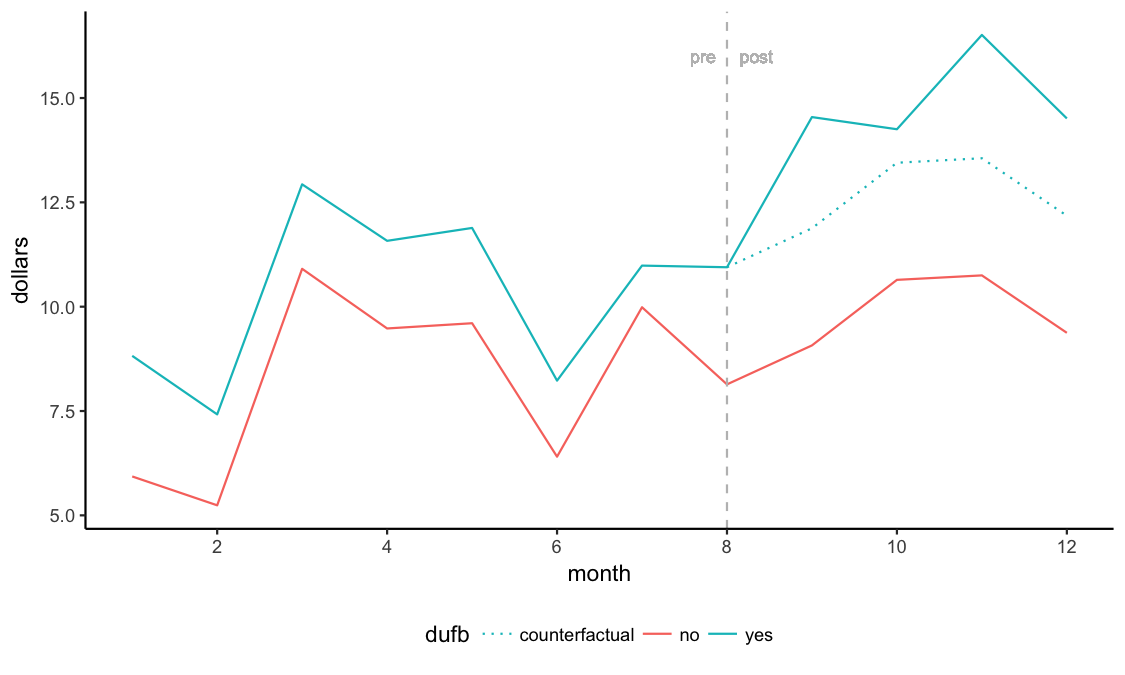
\includegraphics{noriega-prospectus_files/figure-latex/plot-dd-1.pdf}
\caption{\label{fig:plot-dd}Example of Hypothetical Result (Fake Data}
\end{figure}

Displayed in Figure \ref{fig:plot-dd} reflects what I'm hoping to find.
Note that the data is fake and the time interval is by month (I plan to
use daily data). The point of the graph is to emphasis that I expect to
find a jump in dollars spent on fruits and vegetables in the DUFB
(treated) stores once the DUFB program begins in August. While I intend
to use a difference-in-difference-in-differences (DDD) model as part of
my analysis, I display a difference-in-differences (DD) to highlight the
effect of interest.

Assume that the DD displayed is isolating the subpopulation of SNAP
transactions observed. Then the dotted green line beginning at month
\texttt{8} would represent the gap under the ``parallel trends''
assumption. The difference between the solid green line and the dotted
green line represents the increase in dollars spent that I hope to
identify.

\newpage

\hypertarget{data-1}{\section*{Data Description}\label{data-1}}
\addcontentsline{toc}{section}{Data Description}

These data come from a large grocery distributor and retailer serving
multiple grocery chains. Three years of data will be available, 2014
through 2016. To my understanding, this includes months where the DUFB
incentive is active (Aug 1 to Dec 31) and inactive (Jan 1 to July 31)
across all stores. These data are transaction level data and will
include (at least) store number, register, transaction ID, date and time
of purchase, payment type, item, dollars, and quantity.

Double Up implementation occurred in single grocery chain. The chain has
more than 60 stores; 17 were selected as ``treatment'' stores (with
Double Up). Of the remaining stores, data is available from an addition
15 to serve as ``controls''. The quotes here signify that these are
reference terms. The terminology is somewhat misleading; the use of
``treatment'' and ``control'' could lead one to think store assignment
was random. It was not.

\subsection*{How the DUFB Incentive is
Implemented}\label{how-the-dufb-incentive-is-implemented}
\addcontentsline{toc}{subsection}{How the DUFB Incentive is Implemented}

The DUFB incentive can differ in implementation. I know of three
different implementations: earn/redeem DUFB points via loyalty card,
single-use paper coupon, and immediate discount. The earn/redeem DUFB
point system is unique to the retailer that provided these data. For
information on the other two DUFB implementations, see
\citep{margaret_schnuck_doubling_2016}.

The DUFB implementation for this particular grocery store chain is a
point system. SNAP shoppers can \emph{earn} points by buying locally
grown produce using their SNAP EBT card and their loyalty card. Earning
DUFB points requires using a loyalty card. The retailer uses the cards
to keeps track of points. Each dollar spent buying locally grown produce
earns a DUFB point. SNAP shoppers are eligible to receive up to \$20
dollars worth of DUFB points (20 points) per day. Earned points are not
immediately reflected on loyalty cards. They are redeemable the day
after.

Shoppers can redeem points on \emph{any} eligible produce (excludes
frozen and canned fruits and vegetables). Spending SNAP EBT benefits is
not required to redeem points; redeeming points is possible using any
method of payment (tender).

This earn/redeem DUFB point system has four important details. I already
mentioned the first but it's worth reiterating: it takes a day to
process earned points. This forces SNAP shoppers to delay the reward of
the DUFB incentive earned by at least a day. While perhaps a
technological necessity (it takes time to process and reflect earned
points on loyalty card accounts), this delays the earning any of
transactional utility for the SNAP shopper \citep{thaler_mental_1985}. I
expect that delaying transactional utility reduces the ``pleasure'' and
effectiveness window of the DUFB incentive. SNAP shoppers tend to spend
benefits in one large shopping trip soon after receiving monthly
benefits. These shopping trips correspond to the single largest
opportunity to earn DUFB points. These infrequent SNAP shoppers have
limited opportunities to experience the rewarding feedback of redeeming
points. But frequent, salient, rewarding feedback is necessary for habit
formation.

Second, the incentive alternates between earning and redeeming states. A
loyalty card with a DUFB point balance of zero is in an ``earning''
state. After earning DUFB points by buying \emph{locally} grown fresh
produce, the card switches to a ``redeeming'' state; loyalty cards with
a point balance greater than zero will redeem until the point balance is
once again zero. This removes the possibility of strategically
``banking'' earned points. Some shoppers, for example, may want to
``bank'' points then strategically redeemed them all at once (say for a
holiday shopping trip). If I buy 10 dollars of local produce and earn 10
points, then I will continue to redeem points on \emph{any} produce
(even local produce) until the 10 points are gone.

Third, the points \emph{earned} are not communicated to the shopper at
the moment of sale \citep{family_fare_double_2016}. In other words, the
fact that shoppers are earning points is \emph{not salient}. No feedback
exists to connect buying fresh healthy produce to earning points.
Available points (those processed in prior shopping trips) are printed
at the bottom of each receipt, and can even be checked on-line or on
in-store kiosks. But no feedback or information is shared with the
shopper during the current sale. Earning points, at least, ends up being
like any other shopping trip. I would argue this is more a con than a
pro. Certainly a bell shouldn't ring when SNAP shoppers earn points. One
of the great consequences of moving to an EBT card is that the potential
stigma of using food stamps has greatly diminished. But shoppers could
benefit from some sort of feedback that is informative without producing
a spotlighting or stigmatizing effect. For example, shoppers could be
told, ``You saved \$4.50 today and you also earned 5 DUFB
points''.\footnote{I need to confirm that this does not happen.
  Considering the points earned don't appear on receipt, I do not see
  how the clerk know to inform the customer. Does it appear on the
  machine?}

The fourth, and most important point, is that the automatic earning and
redeeming of DUFB points implies that the incentive only works if
individuals choose to actively participate in the program. This is
distinct to standard experimental procedure where individuals are
knowingly assigned to the treatment or control group.

\subsubsection*{\texorpdfstring{What is a ``participant'' for this DUFB
implementation?}{What is a participant for this DUFB implementation?}}\label{what-is-a-participant-for-this-dufb-implementation}
\addcontentsline{toc}{subsubsection}{What is a ``participant'' for this
DUFB implementation?}

How a participant responds to assignment is generally referred to as
\emph{compliance} \citep{angrist_mostly_2008}.\footnote{Participants can
  be further categorized into ``compliers'', ``never-takers'',
  ``always-takers'', and ``defiers''. These categorizations provide
  useful terminology but are not relevant in the context of the DUFB
  incentive.} But in this case, the stores, not the individual shoppers,
have been ``assigned'' to a treatment or control group. Stores, if
assigned to the treatment group by the retail chain, are ``compliers''
by default; the store's point-of-sale (POS) system is altered to
implement DUFB. Some stores (4) behaved somewhat like ``always-takers'',
having asked to participate in DUFB, but most store (13) are
``compliers''.\footnote{I must note that, while this creates some
  worries of ``self-selection'' by stores, I think this bias can be
  handled by a model that includes a store-level fixed-effect.}

How, then, does one think about SNAP shopper participation in the DUFB
program if it is stores that are ultimately assigned to the DUFB
program? SNAP shoppers have the option to benefit from the program
without ever being ``assigned'' to any treatment group. A shopper's
active participation in DUFB is therefore driven by another type of
self-selection. I imagine use of the DUFB incentive depends on a series
latent variables corresponding to individual shoppers, stores, and the
retail chain. For example, demographics, price sensitivity, food
preferences, health consciousness are all latent variables that could
affect shopper DUFB activity. Other latent variables include how
effectively the retail chain markets the DUFB program to the management
of participating stores and how effectively this information is then
relayed to individual shoppers. Management's enthusiasm for the program
is likewise a latent retail chain and store-level variable.

Automatic redemption of the DUFB points also complicates identifying
individual participation. Automatic redemption of DUFB ``points'' means
I cannot identify which SNAP transactions are responding to the
incentive versus ``shopping as usual''. That is, I will observe many
SNAP transactions earning or redeeming DUFB points for fruits and
vegetables that are oblivious to the existence of the incentive. I will
also observe individuals who have chosen to actively participate in the
program. In aggregate, however, I assume that any increase in the total
amount of fruit and vegetables purchases in DUFB stores can be
attributed to the incentive. This is where having purchasing data from
the non-DUFB stores is important. The non-DUFB stores will help improve
estimation by controlling for any changes in fruit and purchases that
may occur for reasons other than the DUFB incentive e.g.~seasonal or
macroeconomic conditions.

\subsection*{Purchases Cannot Be Linked to Individuals (No Loyalty Card
Data)}\label{purchases-cannot-be-linked-to-individuals-no-loyalty-card-data}
\addcontentsline{toc}{subsection}{Purchases Cannot Be Linked to
Individuals (No Loyalty Card Data)}

One important variable that will not be made available is a variable for
loyalty card numbers. The company's use of loyalty cards across its many
chains was an exciting prospect. Previous transaction data from smaller
independent grocery chains had no of way linking purchases to a single
unique identifier over time because these smaller chains did not have
advanced point-of-sale systems.

In earlier conversations with the company, it was understood that
loyalty cards would be made available. However, months into working with
the company, I was informed that this was no longer possible. Per the
company's legal department, the company cannot share any personal
information about their customers. Unfortunately for us, in the loyalty
card contract signed by customers, the loyalty card number itself is
considered personal information, meaning loyalty card numbers fall under
the same legal category as phone numbers and home addresses.

\subsection*{DUFB Incentive Inconsistency Across
Years}\label{dufb-incentive-inconsistency-across-years}
\addcontentsline{toc}{subsection}{DUFB Incentive Inconsistency Across
Years}

The retail company informed us that the way the DUFB incentive worked in
2016 is distinct from 2014 and 2015. The DUFB incentive in 2016 worked
by earning points for each dollar spent on \emph{locally grown} fresh
produce. (Recall that each point is equal to one dollar.) Points are
then redeemed automatically on \emph{any} fresh produce. However, in
2014 and 2015, the incentive was the \emph{opposite}. In those two
years, the DUFB incentive worked by earning points on \emph{any} fresh
produce, automatically redeeming points on \emph{locally grown} fresh
produce.

This is important because \emph{locally grown} fresh produce is a much
smaller subset than \emph{any} fresh produce. Therefore, in years 2014
and 2015, shoppers could easily earn points but had a constrained set of
produce on which to redeem points. In any case, estimates of the
incentive for the year 2015 cannot be compared to estimates in the year
2016.

\subsection*{Limited Dependent
Variable}\label{limited-dependent-variable}
\addcontentsline{toc}{subsection}{Limited Dependent Variable}

For any recorded visit to the cashier---what I call a
``transaction''---there is a good chance a customer does not purchase
fresh fruits or vegetables (FV). If I split a customer's items purchased
during a transaction into a dozen or so general categories (e.g.~dairy,
candy, meat, etc.) and aggregated expenditure over these categories, I
will observe a non-trivial amount of zeros. More importantly, these are
``true'' zeros aka \emph{corner solutions}. That is, these zeros are not
substitutes for missing data or representing negative values but the
result of a utility-maximizing choice.

I cover these concerns in greater detail in the
\protect\hyperlink{methods-1}{Methods Section}.

\subsection*{Other Information}\label{other-information}
\addcontentsline{toc}{subsection}{Other Information}

\textbf{Past Experience with Similar Data}

This is not my first experience working with transaction data. At this
point, I have more than 3 years working with transaction data.
Furthermore, this is not my first experience with transaction data that
includes DUFB transactions and where purchases were not linked to
individuals.

I performed an analysis in April of 2016 for FFN using 5 months of
transaction data from 3 small Detroit-area grocery stores. I produced
Figure \ref{fig:trx-cycle} with these data. It was easy to distinguish
when SNAP benefits were being used in those data. Likewise, it was easy
to tell when transaction made use of the DUFB incentive (either an
issuing of DUFB or a redemption). A simple aggregation could determine
the total amount of dollars spent per some unit time (\emph{day} was the
smallest possible unit of time). I expected data for my prospectus will
be very similar. The empirical models in the next section were developed
under these expectations of the data.

\textbf{SNAP Spending is Cyclical}

In some prior work, I've observed that SNAP spending is cyclical,
peeking in the 2nd week. I expect this was due to the state's monthly
SNAP benefits transfer schedule. Benefits are distributed every odd day
of the month between the 3rd and 21st. Each day maps to the digits
\texttt{0} through \texttt{9}. SNAP participants receive their benefits
once a month on the day corresponding to the last digit of their SNAP ID
number. For example, ID numbers that end in \texttt{0} receive their
benefits on the 3rd of each month. Prior research has found that SNAP
EBT benefits are spent quickly. I stipulate that this is why I observed
fewer SNAP purchases during the 4th week of the month. And fewer SNAP
benefits means fewer transaction capable of receiving the DUFB
incentive. I'm not yet sure what impact this will have on my analysis
this time around, but I thought it important and interesting to point
out and consider.

\begin{figure}

{\centering 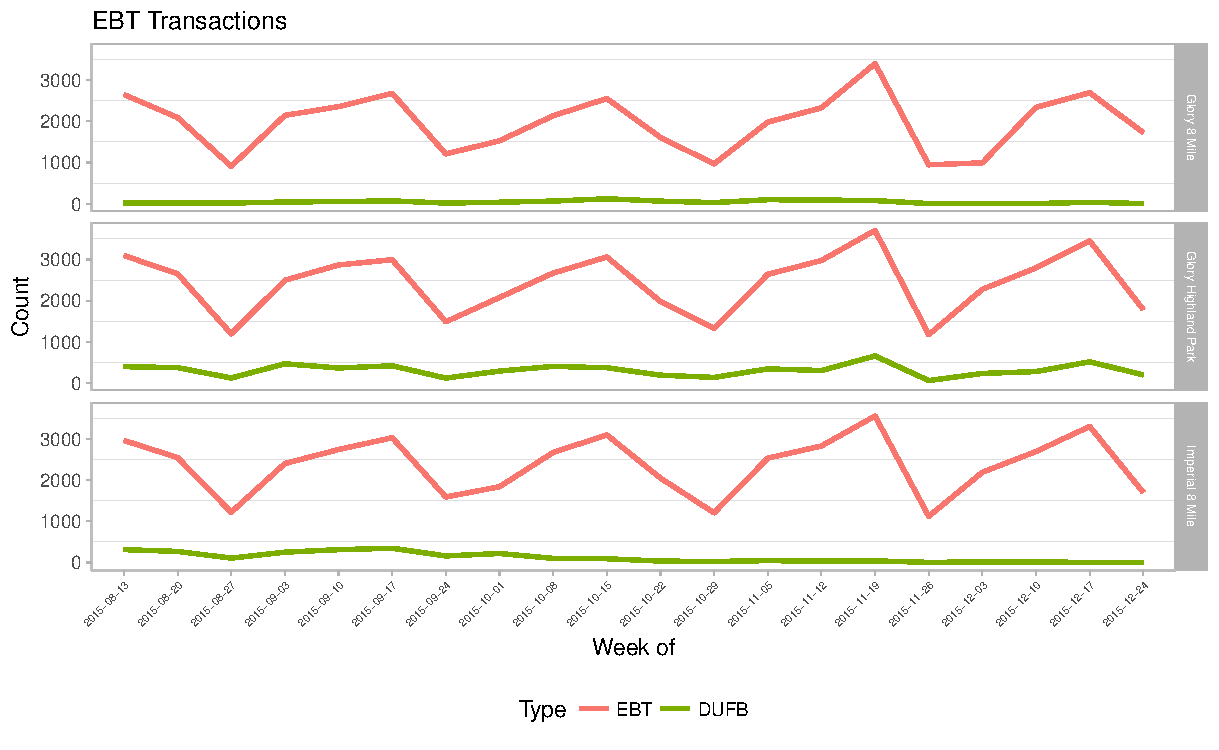
\includegraphics{figures/trx_counts} 

}

\caption{Example of how SNAP EBT benefits are spent in a predicable, week-to-week, cycle. It is the result of how benefits are distributed (uniformly across the first 3 weeks) and of how most SNAP participants spend their benefits (quickly and soon after being received). The red line is the count of transactions where SNAP EBT benefits were used as tender. Ignore the green line.}\label{fig:trx-cycle}
\end{figure}

The week-to-week cyclical pattern of SNAP EBT spending can be observed
in Figure \ref{fig:trx-cycle}. (Note that these are from a different
data source and different store chain, but from the same US state.) At
the start of the each month, SNAP EBT transactions (red line) increase
until peeking at the second week. The count then declines steadily
through the 4th week before once again spiking during the 1st week of
the following month. (Ignore the green line; these are DUFB counts from
a different data set.)

\textbf{Supply Chain Concerns}

One concern I had was if local supply of produce differed geographically
across the state where the stores are located. The company
representative told me that should not be a factor because all stores
are supplied from the same warehouse. Therefore, in theory, each store
should have the same local produce. I plan to visit the stores on a
later date to confirm that this is actually the case.

\hypertarget{store-selection-1}{\section*{Overview of Store Selection
and Expansion}\label{store-selection-1}}
\addcontentsline{toc}{section}{Overview of Store Selection and
Expansion}

How the 17 ``treatment'' stores and 15 ``control'' stores were selected
in 2016 is important. First and foremost, selection was \emph{not}
random. Stores were either selected by the company (13 of 17) or
self-selected into DUFB (4 of 17). Second, the 15 control stores were
selected \emph{after} the selection of the 17 treatment stores. Data
from all remaining stores was requested but the request was denied; only
15 stores had been approved by the company's management. Finally, and
most importantly, the selection criteria for the 17 treatment stores is
\emph{observable}. The implications of this will be covered in more
detail in the \protect\hyperlink{methods}{Methods} section.

\subsection*{Selection and Expansion of DUFB
Stores}\label{selection-and-expansion-of-dufb-stores}
\addcontentsline{toc}{subsection}{Selection and Expansion of DUFB
Stores}

The first 2 stores were piloted with DUFB in 2014. Both were in
geographically distinct areas (these will be referred to as
``\texttt{Node\ 0}'' and ``\texttt{Node\ 1}''). There was a small
expansion adding 3 more stores in 2015. The 3 stores were selected
because they were geographically close to the 2 original pilot stores (2
close to \texttt{Node\ 0}, 1 close to \texttt{Node\ 1}). The 5 stores
are referred to as the ``core''. The location of these 5 stores,
separated in two clusters, established the geographic constraints that
were then used to determine most of the additional stores in 2016.

DUFB was expanded to 12 more stores in 2016, totaling 17. Of those 12, 6
were selected due to their proximity to the 5 core stores, their SNAP
EBT\footnote{Electronic Benefit Transfer.} sales figures, and similarity
in surrounding demographics (high population density, more
African-American). In other words, 9 of the 17 stores---excluding the
initial 2 pilot stores-----were selected on a set of \emph{observable}
characteristics. The remaining 6 stores were not.

Of the remaining 6 stores, 4 asked if they could be included in the
program. These stores \emph{self-selected} into DUFB, making these
stores fundamentally distinct. They were considered, and then included,
only because they fell within the ``Top 50''. The final 2 stores were
selected by the company for ``strategic business decision''. The best
interpretation of this is that the company thought that DUFB would
provide a competitive edge to the 2 included stores given some internal
calculus. How the company came to this decision is \emph{unknown} and
therefore \emph{unobserved}.

Table \ref{tab:store-class} helps understand the year by year expansion
of DUFB. Stores are classified as either \texttt{assigned},
\texttt{self-selected}, or \texttt{unobserved}. To be \texttt{assigned}
means a stores participation in DUFB was determined (assigned) by the
company; \texttt{self-selected} means the store asked the company to
participate; \texttt{unobserved} means that the company selected the
store to participate in DUFB but for unknown and unobserved reasons.
Numbers were assigned to each store for easy reference but otherwise
have no meaningful interpretation.

\begin{table}

\caption{\label{tab:store-class}Year by Year Store Selection. Stores 1 and 2 represent the initial 2014 pilot stores.}
\centering
\begin{tabular}[t]{rlll}
\toprule
Store & 2014 & 2015 & 2016\\
\midrule
1 & pilot & pilot & pilot\\
2 & pilot & pilot & pilot\\
3 &  & assigned & assigned\\
4 &  & assigned & assigned\\
5 &  & assigned & assigned\\
\addlinespace
6 &  &  & assigned\\
7 &  &  & assigned\\
8 &  &  & assigned\\
9 &  &  & assigned\\
10 &  &  & assigned\\
\addlinespace
11 &  &  & assigned\\
12 &  &  & self-selected\\
13 &  &  & self-selected\\
14 &  &  & self-selected\\
15 &  &  & self-selected\\
\addlinespace
16 &  &  & unobserved\\
17 &  &  & unobserved\\
\bottomrule
\end{tabular}
\end{table}

\subsection*{Expansion on Observables}\label{expansion-on-observables}
\addcontentsline{toc}{subsection}{Expansion on Observables}

An example expansion on \emph{observables} (using fake data) can be seen
in Figure \ref{fig:dufb-expansion}. In the top frame, one can see two
blue dots. These blue dots simulate the first two pilot stores in 2014.
The left blue dot is \texttt{Node\ 0} and the right blue dot is
\texttt{Node\ 1}. The gray zones represent areas of higher population
density. Dark gray is considered \emph{urban}, defined as having a
population density of 1500 persons or more per square mile. The light
gray are small towns and cities, more densely populated than very rural
areas, but could not be considered \emph{urban}. The expansion in 2015
(middle frame) proceeds to the stores closest to the original pilot
stores. The expansion continues to 6 more stores in 2016 (bottom frame)
away from the nodes but also along areas of higher population density.

Not conveyed in Figure \ref{fig:dufb-expansion} is that the 2015 and
2016 expansions also move through stores that happen to be ``highly
ranked''---that is, have relatively higher SNAP EBT sales.\footnote{All
  stores within the chain were ranked by SNAP EBT sales as a percentage
  of total sales.} Also not conveyed is the fact that there is a strong
correlation between geography, population density, racial composition,
and SNAP EBT sales. The 2015 expansion to the most nearby stores also
meant that it was an expansion to stores with high SNAP EBT sales in
densely populated, African-American neighborhoods. The 2016 DUFB
expansion was more explicit given that set of feasible stores
substantially increases as one moves away from each node. DUFB stores
were thus specifically selected not just by geographic proximity, but
also by SNAP EBT sales ranking and demographic compositions similar to
the initial 2014 stores.

\textbf{Expansion Data}

Data for about each store was built by merging 4 different sources. The
core data came from the grocery retailer directly, which provided a list
of stores participating in DUFB from 2014 - 2016. The grocery retailer
also provided a list of stores ranked by EBT sales as a fraction of
total store sales and the size (square footage) of each store.
Demographic and socioeconomic data came from the
\href{http://www.datasciencetoolkit.org/}{Data Science Toolkit API}
(DSTK) and the
\href{http://www.census.gov/data/developers/data-sets/acs-survey-5-year-data.html}{American
Communities Survey API} (ACS). The DSTK API provides access to US Census
data from 2000 at the \emph{census block} level and the ACS API provides
data spanning 2010 - 2014 at the \emph{zip code} level. Lastly, data was
extract by mining the
\href{https://www.shopfamilyfare.com/store-locator}{Family Fare}
website.

Matching was done with the ACS data. The ACS zip code data was preferred
because it provided income and housing data. Zip code level demographics
are sufficiently descriptive; stores are evenly distributed across zip
codes. Specifically, 58 stores are spread across 58 zip codes and 4
stores split between 2 zip codes (60 zip codes and 62 stores).\footnote{I
  must also admit that my spatial and geocoding skills improved
  drastically in the months following the matching process. At the time,
  I did not know how determine census blocks from lat/long coordinates,
  relying on the DSTK API that did the conversion. The downside is that
  it returned 2010 data. I'm confident I could do it now, but I still
  think it's not worth the effort given the US Census Data excludes
  income data.}

Ideally, prior to matching, demographic data from the neighborhoods
surrounding the store, who shopped at the store, and how the store was
performing, its size, and goods made available would be known.
Unfortunately, most of the publicly available data was not
store-specific. The only store-specific data came either from the retail
parent company directly or from mining the website.

\begin{figure}

{\centering 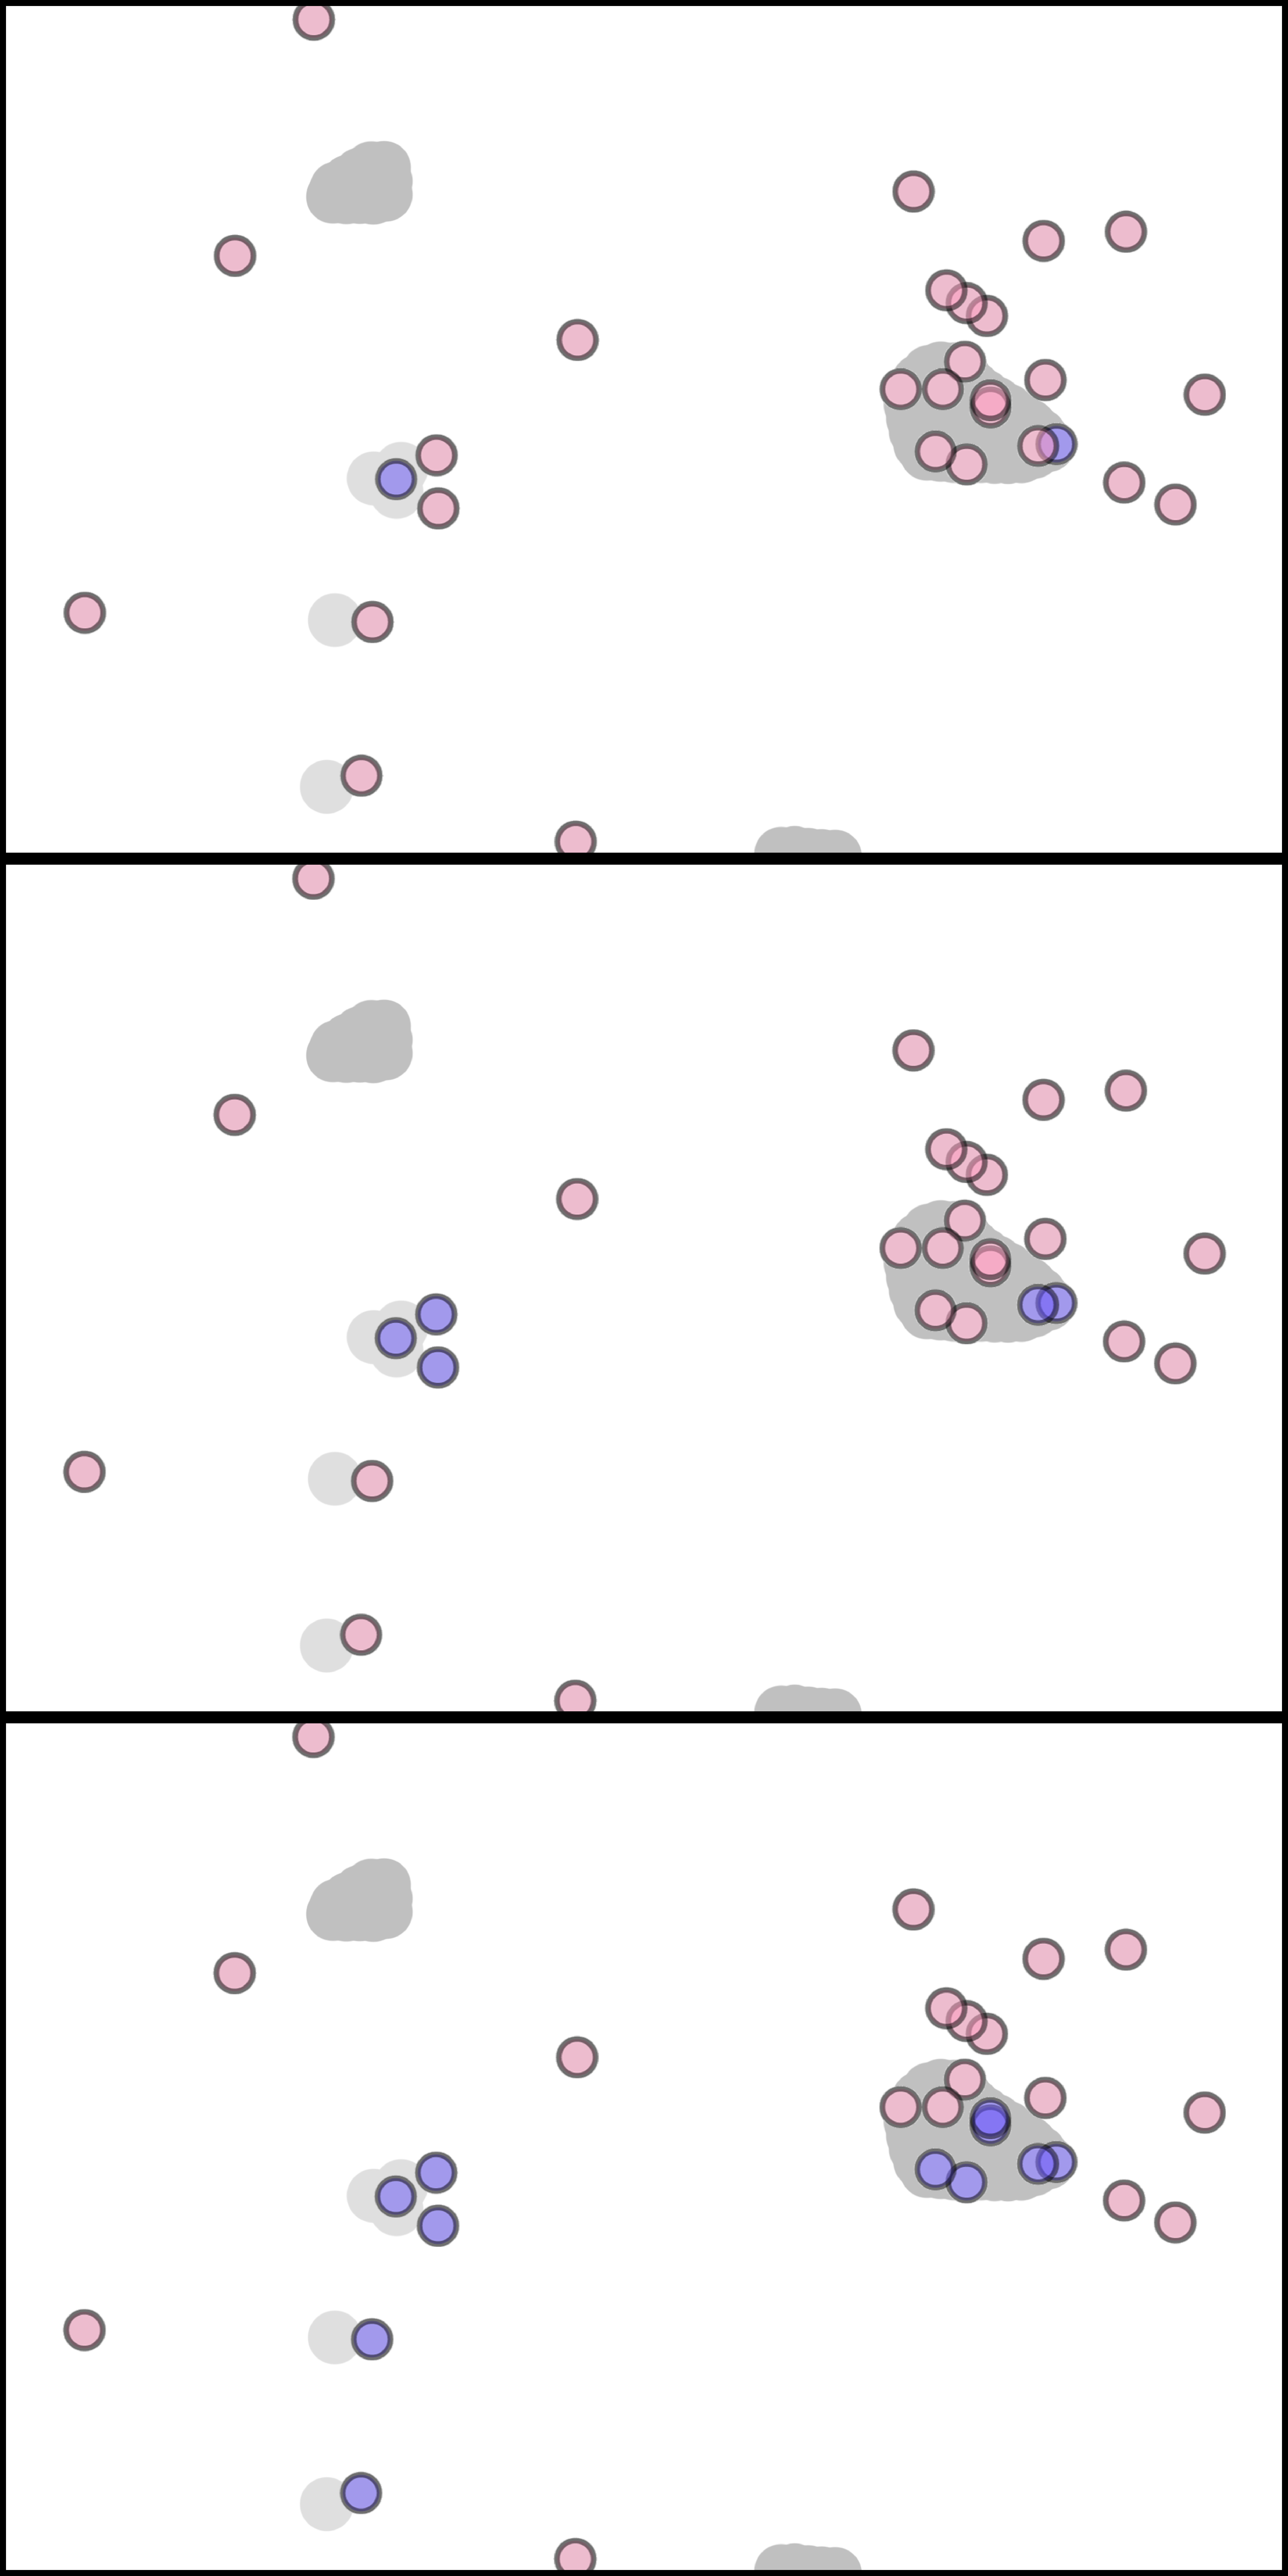
\includegraphics{figures/expansion-v} 

}

\caption{Example expansion over time from 2014 to 2016 (top to bottom) using fake data. Blue dots denote stores with DUFB, pink dots denote without. Gray sectors denote higher population density. The initial nodes can be seen in the top (2014) frame.}\label{fig:dufb-expansion}
\end{figure}

\subsection*{Selection of Control
Stores}\label{selection-of-control-stores}
\addcontentsline{toc}{subsection}{Selection of Control Stores}

Ideally, all remaining stores would have been available to use as a
control group but the company only approved that data be released for 15
stores. This left the added---and incredibly important---step of
selecting the control stores since the company approved, but did not
explicitly select, the 15 stores.

Selecting the control stores proceeded in two steps. First, stores that
either self-selected or were selected using some unobservable criteria
were matched using \emph{Coarsened Exact Matching} (CEM)
\citep{iacus_causal_2011}. Second, stores assigned DUFB were pooled with
nearby control stores and then scored using a linear probability model.
Each step is explained in detail.

\emph{Step 1: Coarsened Exact Matching}

The 6 stores classified as \texttt{self-selected} or \texttt{unobserved}
(stores \texttt{12} through \texttt{17}; see Table
\ref{tab:store-class}) were compared against all possible control stores
for matches. Matching was done across 5 dimensions: race, income,
population density, store attributes, store EBT sales. One variable per
dimension was selected: percentage of population that is
African-American (zip code level); people per square mile (zip code
level); median income for people who have received SNAP or similar
assistance (zip code level); the number of associates employed in each
store; and the percentage of total stores sales attributed to EBT/SNAP.

Of the 6 stores (stores \texttt{12} - \texttt{17}), only 3 produced
viable matches. However, each of the 3 matched stores had matched to
more than one control stores. The closest stores, by driving distance,
were selected as the tie-breaker for each matched store. Stores were
sufficiently far apart, with very sparsely populated areas between, that
``spill-over'' was considered unlikely. That is, it is considered
unlikely that a shopper near a store without DUFB would opt to drive 30
or more minutes to shop at the store \emph{with} DUFB.

This left 12 stores to be allotted to the control group and 3 treatment
stores to be effectively discarded.

\emph{Step 2: Scoring via Linear Probability Model}

Assignment to treatment and control can be perfectly determined since we
know and observe the criteria used for assignment: geographic distance
from an initial store (node), SNAP EBT sales rank, and
demographics---specifically population density and percentage
African-American.\footnote{It should be noted that the company did not
  explicitly say population and race were part of the selection
  criteria. Instead, they said something along the lines of ``stores
  serving a similar population as the original stores.''} A scoring
function was created by fitting a linear probability model to all stores
within 140 kilometers of the two initial pilot stores.

\[
\begin{aligned}
  \bm{s}  &= \widehat{P(\mathbf{D} = 1 | \bm{X}, \bm{N})} \\
          &= \mathbf{X} \bm{\hat \beta} + \hat \alpha \mathbf{N} + \left (\mathbf{X} \odot \mathbf{N} \right ) \bm{\hat \gamma}
\end{aligned}
\]

\(\bm{s}\) are the fitted values of the estimated linear probability
model; \(\mathbf{D} \in \{0,1 \}\) is a \(n \times 1\) vector of store
assignments to DUFB; \(\mathbf{X}\) is an \(n \times k\) matrix of
normalized observable covariates that determine assignment;
\(\mathbf{N} \in \{0, 1 \}\) is an \(n \times 1\) dummy vector denoting
the closest pilot store aka ``Node'', where \(0\) is \texttt{Node\ 0}
and \(1\) is \texttt{Node\ 1}. \(\odot\) represents element-wise
multiplication aka ``Hadamard product''.

Stores were sorted by the fitted values of the model, \(\bm{s}\). There
is perfect separation between DUFB stores and those without (see Figure
\ref{fig:score-plot}). Therefore, the top 11 stores by score value are
all DUFB stores. The next 12 stores by score value are then allotted to
the control group.

\begin{figure}
\centering
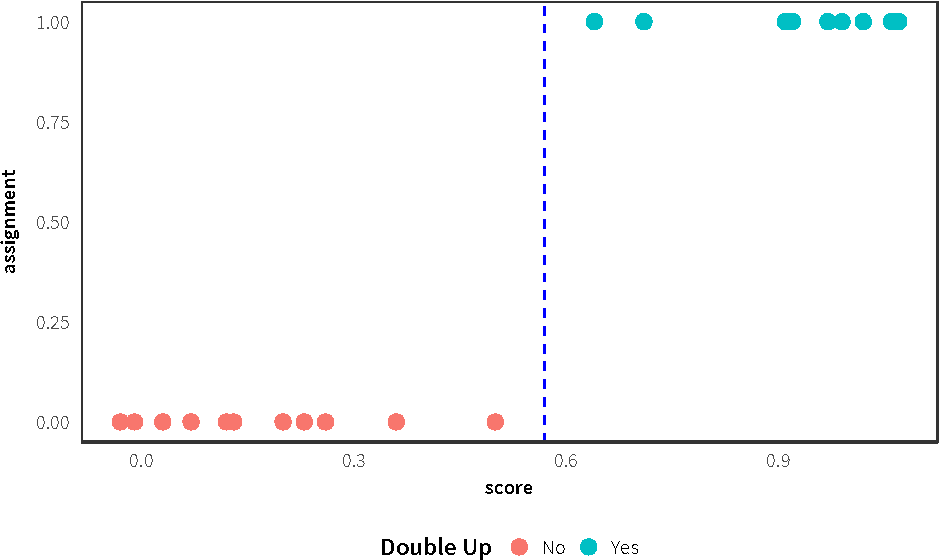
\includegraphics{noriega-prospectus_files/figure-latex/score-plot-1.pdf}
\caption{\label{fig:score-plot}Store Score vs DUFB Assignment}
\end{figure}

\subsection*{Motivation for Matching}\label{motivation-for-matching}
\addcontentsline{toc}{subsection}{Motivation for Matching}

Not all treated stores will be matched to a control. As mentioned, this
is due to the nature of how the 17 treated stores were selected. The
parent company intentionally selected stores with some of the highest
EBT (aka SNAP Electronic Benefit Transfer (EBT) Card) sales that were
also within relatively similar geographic locations. This reduced the
burden of advertising and implementing DUFB for The parent company. The
unfortunate downside of this implementation is that it effectively
removed any likely matches for treated stores located in the most Urban
areas (e.g.~Grand Rapids and Battle Creek).

Here is an example to illustrate why it is infeasible to matching all
treated stores and instead expand selection algorithmically on
observables. If we calculate the percentage of the population by
\emph{zip code} that is African American then split the data into
treatment and control groups, we get the following:

\begin{verbatim}
#> Difference in Means (Treated - Control) = 7.848600
\end{verbatim}

\begin{verbatim}
#> 
#> Population, % Black (Treated, Top 10):
\end{verbatim}

\begin{verbatim}
#>  [1] 26.060929 21.945444 19.790582 18.880000 18.688795 14.693513 11.857163
#>  [8]  8.531952  5.644237  5.644237
\end{verbatim}

\begin{verbatim}
#> 
#> Population, % Black (Control, Top 10):
\end{verbatim}

\begin{verbatim}
#>  [1] 8.575720 8.141256 7.271242 5.057010 4.613969 4.374678 3.256329
#>  [8] 2.955071 2.676733 2.593660
\end{verbatim}

What these results tell us is how potentially distinct the populations
are within the zip codes containing the treated stores. Sorting
population percentages in descending order, no good match exists within
the control stores for the top 7 treated stores. One variable is the
simplest case; matching only gets more difficult as one brings in more
variables to match.

Considering the separation between some of the treated stores and all of
the control stores, it was prudent to rethink the store selection and
matching strategy.

It must be noted that matching is not a necessary step during every
design phase. It is, in large part, a way to hedge against the
possibility that merely selecting the next top 15 stores by EBT sales
could sour the estimates. Matching a smaller set of treatment stores
against a larger pool of controls can often produce estimates less
sensitive to even the smallest changes in some model specifications
\citep{imbens_causal_2015}. However, other models and tools (like
regression) are in relatively unperturbed by a lack of design-phase
matching, but still benefit from having a larger sample size
\citep{angrist_mostly_2008}.

\subsection*{Matching Details}\label{matching-details}
\addcontentsline{toc}{subsection}{Matching Details}

Like most data-dependent endeavors, the most tedious part of matching
the stores was obtaining enough variables. Once enough data were
obtained, variables were selected on how best they captured data from
the following dimensions:

\begin{itemize}
\tightlist
\item
  Demographics (e.g.~race)
\item
  Income/wealth
\item
  Population density (e.g.~urban vs rural)
\item
  Store attributes
\item
  Store EBT sales
\end{itemize}

One may assume that more variables makes matching easier. This is only
true insofar as it provides one with a large pool of options. It is
still necessary to carefully select how many variables one is using
because matching becomes more and more difficult with each added
variable used. This is especially true with a small sample size.

The matching covariates that were finally selected are:

\begin{itemize}
\tightlist
\item
  \texttt{pct\_black} : Percentage of population that is black (zip code
  level)
\item
  \texttt{dens\_pop} : The population density (people per square mile,
  zip code level)
\item
  \texttt{income\_p50\_snap\_yes} : Median income for people who have
  received SNAP or similar assistance (zip code level)
\item
  \texttt{store\_n\_associates} : The number of associates employed in
  each store.
\item
  \texttt{ebt\_sales\_pct} : Percentage of total stores sales attributed
  to EBT/SNAP.
\end{itemize}

~

\textbf{Results of Match}

\begin{table}

\caption{\label{tab:match-results}CEM Match Matrix}
\centering
\begin{tabular}[t]{lrr}
\toprule
  & G0 & G1\\
\midrule
All & 44 & 17\\
Matched & 14 & 3\\
Unmatched & 30 & 14\\
\bottomrule
\end{tabular}
\end{table}

\texttt{G0} represents the ``control'' group and \texttt{G1} represents
the ``treated'' group. One can observe that 3 ``treated'' stores were
matched to 14 ``control'' stores. Each of the 3 treated stores was
matched to its closest control store by driving distance.

\textbf{Covariate Cut-points}

The CEM procedure depends heavily on the ``cut-points'' selected for
each variable. This is akin to setting the cut-off points when turning a
continuous variable into a categorical variable. For example, when
converting income values from dollars into \texttt{low-}
\texttt{middle-} and \texttt{high-income} groups, at least 4 cut-points
are required (2 of which are the maximum and minimum). What the other 2
cut-points are will greatly affect the match. This leads to the
question, for example, should the cut-points be \texttt{25000} and
\texttt{100000} or perhaps the median and the top 10\%?

For the matches produced, the following cut-points were created.

\begin{verbatim}
#> $pct_black
#> [1]  0  2 10 40
#> 
#> $dens_pop
#> [1]    0  200 1000 5000
#> 
#> $ebt_sales_pct
#> [1] 0.00 1.65 3.00 5.00
#> 
#> $store_n_associates
#> [1]  20  40  60  80 130
#> 
#> $income_p50_snap_yes
#> [1] 12000 18000 25000 40000
\end{verbatim}

Understanding why is best explained using a visualization. Below are
graphs of the variables \texttt{pct\_black} and
\texttt{income\_p50\_snap\_yes} with their corresponding cut-points. The
aim of each cut-point is to balance the creation of reasonably sized
partitions while still marking obvious shifts in the underlying
distribution.

For example, in the first plot (\texttt{pct\_black}), there are clearly
points where the slope dramatically increases --- and then spikes --- in
the percentage of African Americans. But in the second plot, the slope
is more gradual, so the partitioning is aimed more at getting relatively
balanced groups.

\includegraphics{noriega-prospectus_files/figure-latex/unnamed-chunk-8-1.png}

\includegraphics{noriega-prospectus_files/figure-latex/unnamed-chunk-9-1.png}

\hypertarget{methods-1}{\section*{Methods}\label{methods-1}}
\addcontentsline{toc}{section}{Methods}

\subsection*{Set up}\label{set-up}
\addcontentsline{toc}{subsection}{Set up}

Recall the research question of interest---whether the DUFB incentive
increases spending on fresh fruits and vegetables (FV) within stores
participating in the program. The outcome variable, in this case, is
total spending on FV.

I've considered other possible values for the outcome variable. For
example, the proportion of dollars spent per transaction or the total
ounces of FV purchased. Each added an extra layer of complication. Using
proportion of expenditure per given transaction would vary wildly,
particularly with small transactions, and would create two mass points
at zero and one (no FV purchased and only FV purchased). Total ounces
depends on the variable and quality of the data. I cannot be sure the
data received will contain counts or ounces for fresh fruits. Fresh
fruits generally do not have UPC values. Dollars spent (expenditures) on
FV gets to the heart of the question and is guaranteed to be in the
data.

Unfortunately, using the total expenditure of FV is complicated by 3
problems.

\begin{enumerate}
\def\labelenumi{\arabic{enumi}.}
\tightlist
\item
  Purchases not linked to customers.
\item
  Outcome Variable with non-trivial amount of zeros (corner solutions).
\item
  Consumers maximize across multiple product types.
\end{enumerate}

The first problem is not specific to the outcome variable. The inability
to link purchases to individuals means I cannot use Panel Data Methods
at the customer level; I will be unable to look at how customer behavior
changes over-time and cannot control for unobserved customer
heterogeneity. I'm instead limited to methods for repeated
cross-sections over-time.

The second and third problems are directly related to the preferred
outcome variable. I anticipate a non-trivial amount of zeros because I
expect to observe a large fraction of transaction where no FVs are never
purchased. Likewise, FV expenditures are often only part of a basket of
goods. Just as I anticipate a non-trivial amount of zeros, I also
anticipate that FVs are not purchased independently of other goods. When
spending their money, consumers optimize expenditures across a large set
of options. This optimization is also complicated by the first problem
(cannot link) but I will go into more details later.

\subsection*{Methods Overview}\label{methods-overview}
\addcontentsline{toc}{subsection}{Methods Overview}

\textbf{Difference-in-Difference-in-Differences}

I want to measure the difference in SNAP EBT dollars spent or redeemed
on fresh produce. If the incentive is working, then I should see in
increase in SNAP EBT dollars spending on fresh produce within stores
implementing the DUFB incentive. I do not think it's enough to assume
the DUFB incentive, if effective, will be measurable without considering
heterogeneity. That is, if a store's implementation of DUFB affects
individual behavior, the effect could be hard to measure if measured
across the entire distribution of FV purchases, instead of the subset of
SNAP EBT dollars spent.

The Difference-in-Difference-in-Differences (DDD) regression is a
fitting framework if I expect the SNAP population that patrons DUFB
stores to be systematically different from the SNAP population that
patrons the non-DUFB stores.\footnote{See
  \citet{wooldridge_econometric_2010} for more details. I'm assuming
  familiarity with the DDD model.} Differencing along time, store DUFB
group, and the type of transaction (SNAP or not) will reasonably capture
any systematic differences.

This is unfortunately complicated given that I cannot link transaction
to individuals. But I can tell if a purchase was made with SNAP EBT
dollars or that it redeemed DUFB points. This is enough to split
transactions into SNAP/DUFB-redeemed versus other standard transactions.
This provides a way of grouping to perform a DDD.

Any model like DDD that is estimate via OLS, however, ignores the second
and third problems. I think it is prudent to consider consumer choice
behavior and the mechanisms that generate zero-expenditures. Numerous
demand models exists for cross-sectional data that, with a few
assumptions (like each transaction represents a distinct individual),
may better estimate the impact of the DUFB incentive than straight OLS.

There is a vast literature on consumer purchasing behavior aka choice
models (see \citet{train_discrete_2009} for an introductory overview).
Multiple-discrete choice models, in particular, have become popular
given the increased availability of transaction-level (scanner) data
\citep{dube_multiple_2004, hendel_estimating_1999}. Multiple-discrete
choice models, however, are too product-specific. It is not important
for me to model which brand and quality of bananas or carrots were
purchased. What is important to me is how much was spent on bananas,
carrots, and other fruits and vegetable types versus other non-FV types.
Remember, my outcome variable is expenditure on \emph{total} FV
spending. I'm far more concerned about whether or not consumers are
observed buying \emph{any} FV than I am with the exact types. That said,
expenditure on non-FV is also important. \emph{Therefore, I need a model
framework flexible enough to handle a continuous outcome variable with a
non-trivial amount of zeros (corner solutions) and multiple types of
goods.}

\textbf{Continuous Outcome Variables and Corner Solutions}

Corner solutions for expenditures can occur for various reasons.
\citet{pudney_modelling_1989} covers three of the most likely mechanisms
producing ``true'' zeros in cross-sectional data. The first is that the
data was gathered in too short a period of time for the purchase to
occur. This problem is far more common in cross-sectional data of
infrequently purchased goods (i.e.~durable goods like cars or
refrigerators). The second is due to a supply side factor the customer
has no control over. For example, there could be a shortage of FVs or
none are available. Imagine searching for FV purchases in convenience
store data. Many zeros would exists because some convenience stores do
not sell FVs. The third zero results from a customer's decision as a
function of prices, preferences, and income constraints. A zero is
perhaps observed because FVs are too expensive and the customer can get
larger quantities of other, equally or more preferred, foods for the
same price.

I expect the first mechanism could apply to food purchases under
specific circumstances. If data are left disaggregated or the period of
observation is shrunk substantially, zeros for FVs will exists due to
infrequency of purchase. For example, customers that make frequent trips
to the store may not always buy FVs. A cross-section of data from one
day may have a non-zero FV value for the customer but zero the next. The
third mechanism applies very naturally to the grocery store environment
(classical utility theory). The second will require further
verification. I do not expect to find out that there were shortages of
FVs in the stores observed, but I could be wrong.

\citet{humphreys_dealing_2013} and \citet{carlevaro_multiple_2016}
discuss cross sectional models that accommodate corner
solutions---Tobit, \emph{Two-Part}, and \emph{Hurdle} models,
specifically.\footnote{\citet{wooldridge_econometric_2010} does not
  appear to differentiate between ``Two-Part'' models and ``Hurdle''
  models. I will use it following \citet{humphreys_dealing_2013}
  language, which does.} The classic ``corner solution'' regression
model is the Tobit model. Corner solutions are utility maximizing and no
assumptions are made about the decision not to purchase/consume. In
contrast to the Tobit model, the decision to participate in consumption
is explicitly formulated in the Two-Part and Hurdle models.
Participation is the ``first hurdle'', the amount purchased/consumed is
the ``second hurdle''.

In the ``Naive'' Two-Part model, the decision to buy is estimated
separately and sequentially from how much (amount) to buy; Probit is
used to estimate the decision-to-buy process and OLS is used to estimate
the amount purchased. The Double Hurdle model estimates both these
decision simultaneously via maximum likelihood. The full Double Hurdle
model allows for correlation between the error terms in the decision and
amount/consumption equations \citep{jones_note_1992}. Imposing the
assumption that unobservable factors between the decision and amount
decisions are uncorrelated reduces the full ``Jones'' Double Hurdle to
the ``Cragg'' model \citep{cragg_statistical_1971}.

It is unclear to me if Two-Part or the Double Hurdle models that
formalize ``participation'' are necessary when considering FV purchases.
This makes more intuitive sense for something like cigarette or alcohol
consumption, where zero-expenditure can be the result of abstention or
price/income constraints.\footnote{See \citet{garcia_alternative_1996}
  and \citet{aristei_cohort_2008} for abstention-style hurdles.} There
are, after all, consumers who will never consume cigarettes or alcohol,
even if free (abstention). But I'm not sure if an abstention mechanism
is reasonable when considering FV purchases. Do consumers really opt out
(or abstain) from buying FVs altogether?

An infrequency of purchase mechanism for FVs, however, seems more
reasonable. \citet{deaton_statistical_1984} introduced this mechanism as
an expansion to the Tobit model. This Double Hurdle has been used to
model infrequent purchases of butter, pork, and prepared meals
\citep{yen_modeling_1995, su_microeconometric_1996, newman_double-hurdle_2003}.
I find it reasonable to expect that, for any given daily cross-section
of data, some of the zeros observed will be due to infrequent purchase
of FVs.

It's worth noting the general increased popularity of Hurdle models as
alternatives to Tobit, and other related models, like Adjusted Tobit and
Heckit models. There is a long existing debate over which models perform
better, with most of the criticism falling on Tobit. Monte Carlo
comparisons under different error distributions and exclusion
restrictions find Hurdle models consistently out performing Tobit and
Heckit models, both in model fit and coefficient bias
\citep{hay_ordinary_1987, manning_monte_1987}. Monte Carlo studies have
also been used to defend both approaches, encouraging a more flexible,
case-by-case approach on choosing the appropriate model
\citep{leung_choice_1996, dow_choosing_2003, madden_sample_2008}. But
applied work in the applied social science, like health care expenditure
and consumer purchases, generally tend to favor use of Hurdle models
over Tobit or Heckit models
\citep{yen_working_1993, smith_tobit_2003, stewart_tobit_2013}.

\textbf{Multiple Goods}

The limitation of Tobit and other hurdle models is the estimated demand
of a single good. Ideally, expenditure on different types of goods
better captures the decisions and purchasing behavior of customers
within a grocery store. That is, instead of collapsing all expenditure
on FVs into one outcome variable, the model would allow for customers to
optimize across \emph{multiple} goods of different types while also
allowing corner solutions. Multiple discrete choice models allow the
purchase of multiple types of goods, but do not capture the intensive
margin (the amount) of the good purchased/consumed.

\citet{dubin_econometric_1984} construct a \emph{discrete-continuous}
model were consumers can select from multiple goods/options but that
they are mutually exclusive, perfect substitutes. The \emph{discrete}
component of the model captures the decision to buy a non-zero amount;
the \emph{continuous} part captures the amount
purchased/consumed/utility acquired. The mutually exclusive, perfect
substitute condition, however, means that one cannot be observed
buying/consuming more than one good/option.

For any observed trip to the store, zero-expenditure in FV implies
non-zero expenditure for some non-FV. Ignoring this seems unwise and I
plan, at a minimum, to implement a model optimizing along two
dimensions---FV and non-FV. The best model I've found is the
\emph{multiple} discrete-continuous model extreme value (MDCEV) model
introduced by \citet{bhat_multiple_2005}. MDCEV is an extension of the
Kuhn-Tucker based model developed by \citet{wales_estimation_1983}.
MDCEV allows non-zero consumption across multiple goods.
\citet{kim_modeling_2002} solved the intractability of the
\citet{wales_estimation_1983} model. \citet{bhat_multiple_2005}
simplified both to be more realistically applicable.

In the next subsection, I will formally introduce the different modeling
structures I intend to use in my paper. I will first introduce the DDD
framework were estimation via OLS is sufficient. I then expand from OLS
to Tobit and other Hurdle models before expanding into the more complex
MDCEV model. The shared goal, across all models, is the best possible
measurement of the impact the DUFB incentive has on fruit and vegetable
expenditures between participating and non-participating stores.

\begin{center}\rule{0.5\linewidth}{\linethickness}\end{center}

\subsection*{Difference-in-Difference-in-Differences
(DDD)}\label{difference-in-difference-in-differences-ddd}
\addcontentsline{toc}{subsection}{Difference-in-Difference-in-Differences
(DDD)}

I observe transaction \(i=1,...,L\) in store \(j=1,...,N\) across
\(t=1,...,T\) days. Let \(y_{ijt}\) be total FV expenditures for
transaction \(i\) in store \(j\) on day \(t\). The DDD regression is

\[
\begin{aligned}
y_{ijt} &= \alpha_0 + \alpha_1 dE_j + \alpha_2 dS_i  + \alpha_3 dE_j \cdot dS_i \\& \quad + \theta_1 dP_t + \theta_2 dP_t \cdot dE_j + \theta_3 dP_t \cdot dS_i \\
& \quad + \delta dE_j \cdot dS_i \cdot dP_t + \bm{x'}_{ijt} \bm{\beta} + \lambda_t + \epsilon_{ijt}
\end{aligned}
\]

where \(dE_j\) represents store assignment to DUFB group, \(dS_i\)
represents a SNAP or SNAP related transaction (target group), and
\(dP_t\) represent the treatment period, August - December.
\(\lambda_t\) captures daily (time) effects and \(\bm{x'}_{ijt}\) is a
vector of observable characteristics about transaction \(i\) in store
\(j\) on day \(t\). The coefficient of interest is \(\delta\).
\(\epsilon_{ijt}\) are idiosyncratic errors at the transaction level.

Again, I do not observe individuals, only transactions. Yet I think it
reasonable to assume that the structure of daily transaction data more
closely resembles that of repeated cross-sections than of panel data.
Assuming it was possible to link individuals to purchases and build
panel data, the same individual would likely be observed
\emph{sporadically} within in a given month. That is, were this to be
panel of the same \(N\) individual shoppers across \(T\) total days,
many---if not most---of those days would have missing data. There would
certainly be shoppers observed multiple times per week, but I expect
such shoppers to be rare. I certainly would not expect to have a
balanced panel and no shopper would be observed all 365 days.

I therefore find it reasonable to treat each day of observed data as a
single independent cross-section of \(L\) transactions generated by
\(N \le L\) unknown individuals across \(J\) many stores. Aligned
sequentially, these form repeated cross-sections over-time. Each
transaction also falls naturally into a cluster---the store where it
occurred---that is time-invariant and determined prior to the data being
collected.

The model DDD model above can be improved by introducing store effects.
These effectively capture DUFB assignment and all other time-invariant
store-level characteristics. The \(dE\) dummy, for example, drops out.
The notation can also be cleaned up by condensing the other dummies,
emphasizing only variation. The spruced up model is

\begin{equation}
y_{ijt} = \gamma_j + \lambda_t + \phi_0 D_i + \phi_1 D_{ij} + \phi_2 D_{it}+ \phi_3 D_{jt} + \delta_t D_{ijt} + \bm{x'}_{ijt} \bm{\beta} + \epsilon_{ijt}
\label{eq:ddd}
\end{equation}

where \(\gamma_j\) now represents store effects, \(dS_i \equiv D_i\),
and the remaining dummy variables \(D_{ij},~D_{jt},~D_{it},~D_{ijt}\)
represent the dimensions along which they vary---\(i\) transaction type
(SNAP or not), \(j\) store experiment group, and \(t\) day during DUFB
treatment period (August - December). To capture more detail than just
the average, \(\delta_t\) is allowed to vary by day.

\textbf{Unobserved Effects}

I still do not know what the transaction characteristic variables will
be and hence do not know what variables go into \(\bm{x'}_{ijt}\). I do
know, however, that without panel data, I have no methods for dealing
with unobserved individual effects. That is, some unobserved individual
effect \(c_i\) likely exists such that \(e_{ijt} = c_i + u_{ijt}\) where
\(\exists t \ni E[\bm{x'}_{ijt}c_i] \ne 0\). In short, my estimates will
be biased due to an omitted variables problem.

I'm am still thinking about how I can capture part of the unobserved
individual effect \(c_i\). I am open to suggestions.

\begin{center}\rule{0.5\linewidth}{\linethickness}\end{center}

\subsection*{Tobit and other Hurdle
Models}\label{tobit-and-other-hurdle-models}
\addcontentsline{toc}{subsection}{Tobit and other Hurdle Models}

Calculating fruit and vegetable expenditures, \(y_{ijt}\), for each
transaction will result with a non-trivial amount of zeros. These zeros
are not ``censored'' values in the Heckman selection problem sense. They
are genuine zeros aka ``corner solution''. But the mechanisms behind the
zeros is unknown.

\textbf{Tobit Model}

The Tobit model is agnostic to the economic mechanism generating corner
solutions. It is the basic approach when little else is known other than
the decision not to purchase fruits and vegetables is resulting in
zero-expenditures. The basic structure is

\[
\begin{aligned}
y^* &= x'\beta + u \\
y &= max(0, y^*)
\end{aligned}
\]

where \(y^*\) is a latent variable and \(y\) is observed. Tobit can be
generalized beyond requiring homoskedastic error terms but requires
normality. This is important because error terms in repeated cross
sectional data are assumed independent \emph{not} identically
distributed. In other words, heteroskedastic. Other than error term
specifications, any additive and linear-in-parameters regression can be
estimated using Tobit. In other words, I can set \(y^*\) equal to
equation \eqref{eq:ddd}.

For details on the likelihood functions, see \citet{amemiya_tobit_1984}.

\textbf{Hurdle and (Naive) Two-Part Models}

Hurdle models generally have two parts (i.e. ``Double'' Hurdle)---a
decision-to-buy (participate) and the amount to purchase (consumption)
\citep{jones_double-hurdle_1989}. Let \(I^* \in {0,1}\) indicate the
decision to purchase fruits and vegetables and \(y^*\) be the amount of
dollars spent. Both are latent variables. Let \(y\) be observed
expenditures. Formally,

\[
\begin{aligned}
I^* &= z'\gamma + v \\
y^* &= x'\beta + u  \\
y   &= I^* \times max(0, y^*) \\
& \phantom{x}\\
(u,v) & \sim N(0,\Omega) \\
\Omega & = {\left (
\begin{array}{cc}
  \sigma^2_{u} & \sigma_{uv} \\
  \sigma_{uv} & \sigma^2_{v}
\end{array}
\right )}
\end{aligned}
\label{eq:dhurdle}
\]

The \citet{jones_double-hurdle_1989} ``Full'' Double Hurdle model and
the \citet{cragg_statistical_1971} have the same framework. The
distinction is that in the Cragg model assumes no correlation between
\(u\) and \(v\) (i.e. \(\sigma_{uv} = 0\)). The likelihood function for
the Cragg model is, in other words, a simplification of the Jones model.
Formally, the Jones model is

\[
\begin{aligned}
L &= \prod_0
  \left [
    1 - \Phi
    \left (
      \frac{z'\gamma}{\sigma_v},
      \frac{x'\beta}{\sigma_u},
      \rho
    \right )
  \right ] \times \\
& \quad ~ \prod_{+} \Phi
  \left [
      \frac{ \left (
        \frac{z'\gamma}{\sigma_v} +
        \rho(y^* - x'\beta) \right )}
         {\left ( \sqrt{1 - \rho^2} \right ) } \right ]
\frac{1}{\sigma_u} \phi \left ( \frac{y^* - x'\beta}{\sigma_u} \right )
\end{aligned}
\label{eq:lhurdle}
\]

Once again, setting the DDD to be \(y^*\) is not a problem. The main
problem is determining the participation equation \(I^*\). What factors
variables participation i.e.~the decision-to-buy fruits and vegetables?
Variables about individual characteristics would certainly be helpful
here but that isn't possible. Some mechanism is driving consumers to buy
or not buy fruits and vegetables. The likeliest candidate is data on
\emph{other} products purchased within a given transaction. The
existence of complimentary goods (e.g.~olive oil, meats, etc.) may
increase the likelihood of observing FV purchases within the same trip.
The size of the shopping basket likely increases overall chances of FV
purchases. Day of the week or week of the month effects will also
matter, since government benefits and pay schedules may increase the
chances of shopping trips in aggregate.

I anticipate estimating both the Jones and Cragg model as a robustness
check. But I do not expect \(Cov(\sigma_u, \sigma_v) = 0\) given I
cannot capture individual effects. Unobserved individual effects affect
both participation and consumption. In both equations, the error term
absorbs the individual effect, making them correlated by construction.

I will also estimate a ``Naive'' Two-Part model, where the participation
and consumptions equations are estimate independently from the other
(Probit + OLS). Again, just another point of comparison.

\textbf{Multiple Discrete-Continuous Extreme Value Models}

The \citet{bhat_multiple_2005} Multiple Discrete-Continuous Extreme
Value (MDCEV) framework allows for choice along a vector of non-mutually
exclusive goods. Non-negative consumption is allowed across all goods.

I will attempt to use a later iteration of the MDCEV model from
\citet{bhat_multiple_2008}. The distinction that interest me is that the
Bhat (2008) model allows for price variation across goods and explicitly
formulates the Kuhn-Tucker constraints using expenditures. The
econometric model is as follows.

Utility from purchasing vector of goods \(\bm(x) = (x_1, x_2,...,x_k)\)
is defined as

\[
\begin{aligned}
\tilde{U} &= \sum_k \frac{\gamma_k}{\alpha^*_k} \psi(z_k, \epsilon_k)
  \left [
    \left (
      \frac{y_k}{\gamma_k p_k} + 1
    \right )^{\alpha_k} - 1
  \right ] \\
\psi(z_k, \epsilon_k) &= exp(z'_k\beta + \epsilon_k)
\\
\sum_k p_k &= Y
\end{aligned}
\]

where \(z_k\) is a vector of attribute variables about product \(k\) and
of the consumer, \(y_k\) is expenditure on product/good \(k\), \(p_k\)
is the price, and \(Y\) is total expenditure on basket of goods
\(\bm(x)\). \(\epsilon_k\) are idiosyncratic shocks with an
extreme-value distribution. To understand the role of \(\psi_k\),
\(\alpha_k\) and \(\gamma_k\), see \citet{bhat_multiple_2008} for
details.

Using the first good as a reference group, the KT conditions that solve
the optimal expenditure problem (the Lagrangian above) are

\[
\begin{aligned}
V_k^* + \sigma \epsilon_k &= V_1^* + \sigma \epsilon_1 \text{ if }
  y_k^* > 0 (k = 2,3,...,K) \\
V_k^* + \sigma \epsilon_k &< V_1^* + \sigma \epsilon_1 \text{ if }
  y_k^* = 0 (k = 2,3,...,K), \text{ where } \\
V_k^* &= \sigma z'_k \beta + \sigma (\alpha_k - 1)
  \text{ln} \left ( \frac{y_k}{\gamma_k p_k} + 1 \right ) - \text{ln} p_k
\end{aligned}
\]

where \(V_k\) is identified only when \(\alpha_k\) or \(\gamma_k\) is
fixed (both terms estimate related ``satiation'' behaviors). See
\citet{bhat_multiple_2008} (equations 18 and 19) for the Jacobian and
closed form expression for the probability of spending \(y_k^*\).
Example likelihood function to solve the equation for \(i=1,...,L\)
transaction (or \(N\) individuals) in a given cross-section can be found
in \citet{bhat_multiple_2005} (equation 18) and
\citet{bhat_household_2006} (equation 8).

\textbf{Expected Challenges with this Model}

Despite the theoretical advantages of the MDCEV framework
(i.e.~optimization over multiple goods allowing corner solutions), there
are a few challenges I anticipate with using the MDCEV framework.

The first is a concern about prices. The most effective way to
incorporate price variation is to make the basket of available goods
equal to the full universe of observed products. This would likely be
huge. The MDCEV framework is flexible enough to do it, but my fear is
that it will lead to some difficulties in interpretation. In reality,
however, I don't care as much about expenditure at the product level as
much as I do about expenditure on particular types. That is, I care more
about spending on FVs versus non-FVs. Therefore, at the simplest level,
my vector of possible goods would be just 2. However, how would I price
FV versus non-FV? I could construct a price index for just those two
groups but it would combine far too many distinct food types to be
reasonable. Moving towards something like having between 20 to 40
general food categories seems like better approach. For example,
\citet{harding_effect_2014} estimate the prices for 33 different product
groups by using the Stone price index, which depends only on observable
price values.

The second concern is programming related. There are no available
packages that implement the MDCEV package. I would have to adapt the
GAUSS code provided by Bhat on his website in order to get the model
running. This isn't a concern about being able to do it as much as the
amount of time it would require to learn/understand GAUSS in order to
implement it in R or Python.\footnote{It looks like some folks at the
  company \href{http://www.mobilityanalytics.org}{Mobility Analytics}
  have started, which is very promising.}

\begin{center}\rule{0.5\linewidth}{\linethickness}\end{center}

\subsection*{Regression Discontinuity
(RD)}\label{regression-discontinuity-rd}
\addcontentsline{toc}{subsection}{Regression Discontinuity (RD)}

I also plan to perform a secondary Regression Discontinuity (RD) Design
analysis.

In the \protect\hyperlink{store-selection-1}{Store Selection} section, I
discussed the construction of the score function
\(\bm{s} = \widehat{P(\mathbf{D} = 1 | \bm{X}, \bm{N})}\). The score of
each store can be determined via observable data,
\(s_{j} = \widehat{P(D_{j} = 1|\bm{x}_{j}, n_{j})}\). These scores, when
ordered, produced perfect separation between experimental stores and
control stores (see Figure \ref{fig:score-plot2}).

An RD design requires a \emph{running variable} where, above some value
\(c\), the probability of being assigned to the experimental group is
\(1\). Assume I make the score function \(\bm{s}\) my running variable
such that \(D_{j} = \bm{1}[s_{j} \ge c]\).

In my case, assignment \(D_{j}\) is determined by \(s_{j}\) by
construction. Recall that \(s_{j}\) is a function estimated on
observable covariates. These are the same observable covariates the
company used to determine assignment for a subset of stores. I used a
linear probability model to estimate the score function and the
estimated model perfectly predicted assignment. I then ordered stores by
their score value and selected the next 12 unassigned stores.

This problem is that I do not actually know \(c\). I only know that
\(c \in (0.50, 0.64)\). The light gray band in Figure
\ref{fig:score-plot2} displays the possible values of \(c\). The
problem, in essence, is that I do not have---and never will
have---enough stores, so I'm lacking density around where the separation
occurs.

\begin{figure}
\centering
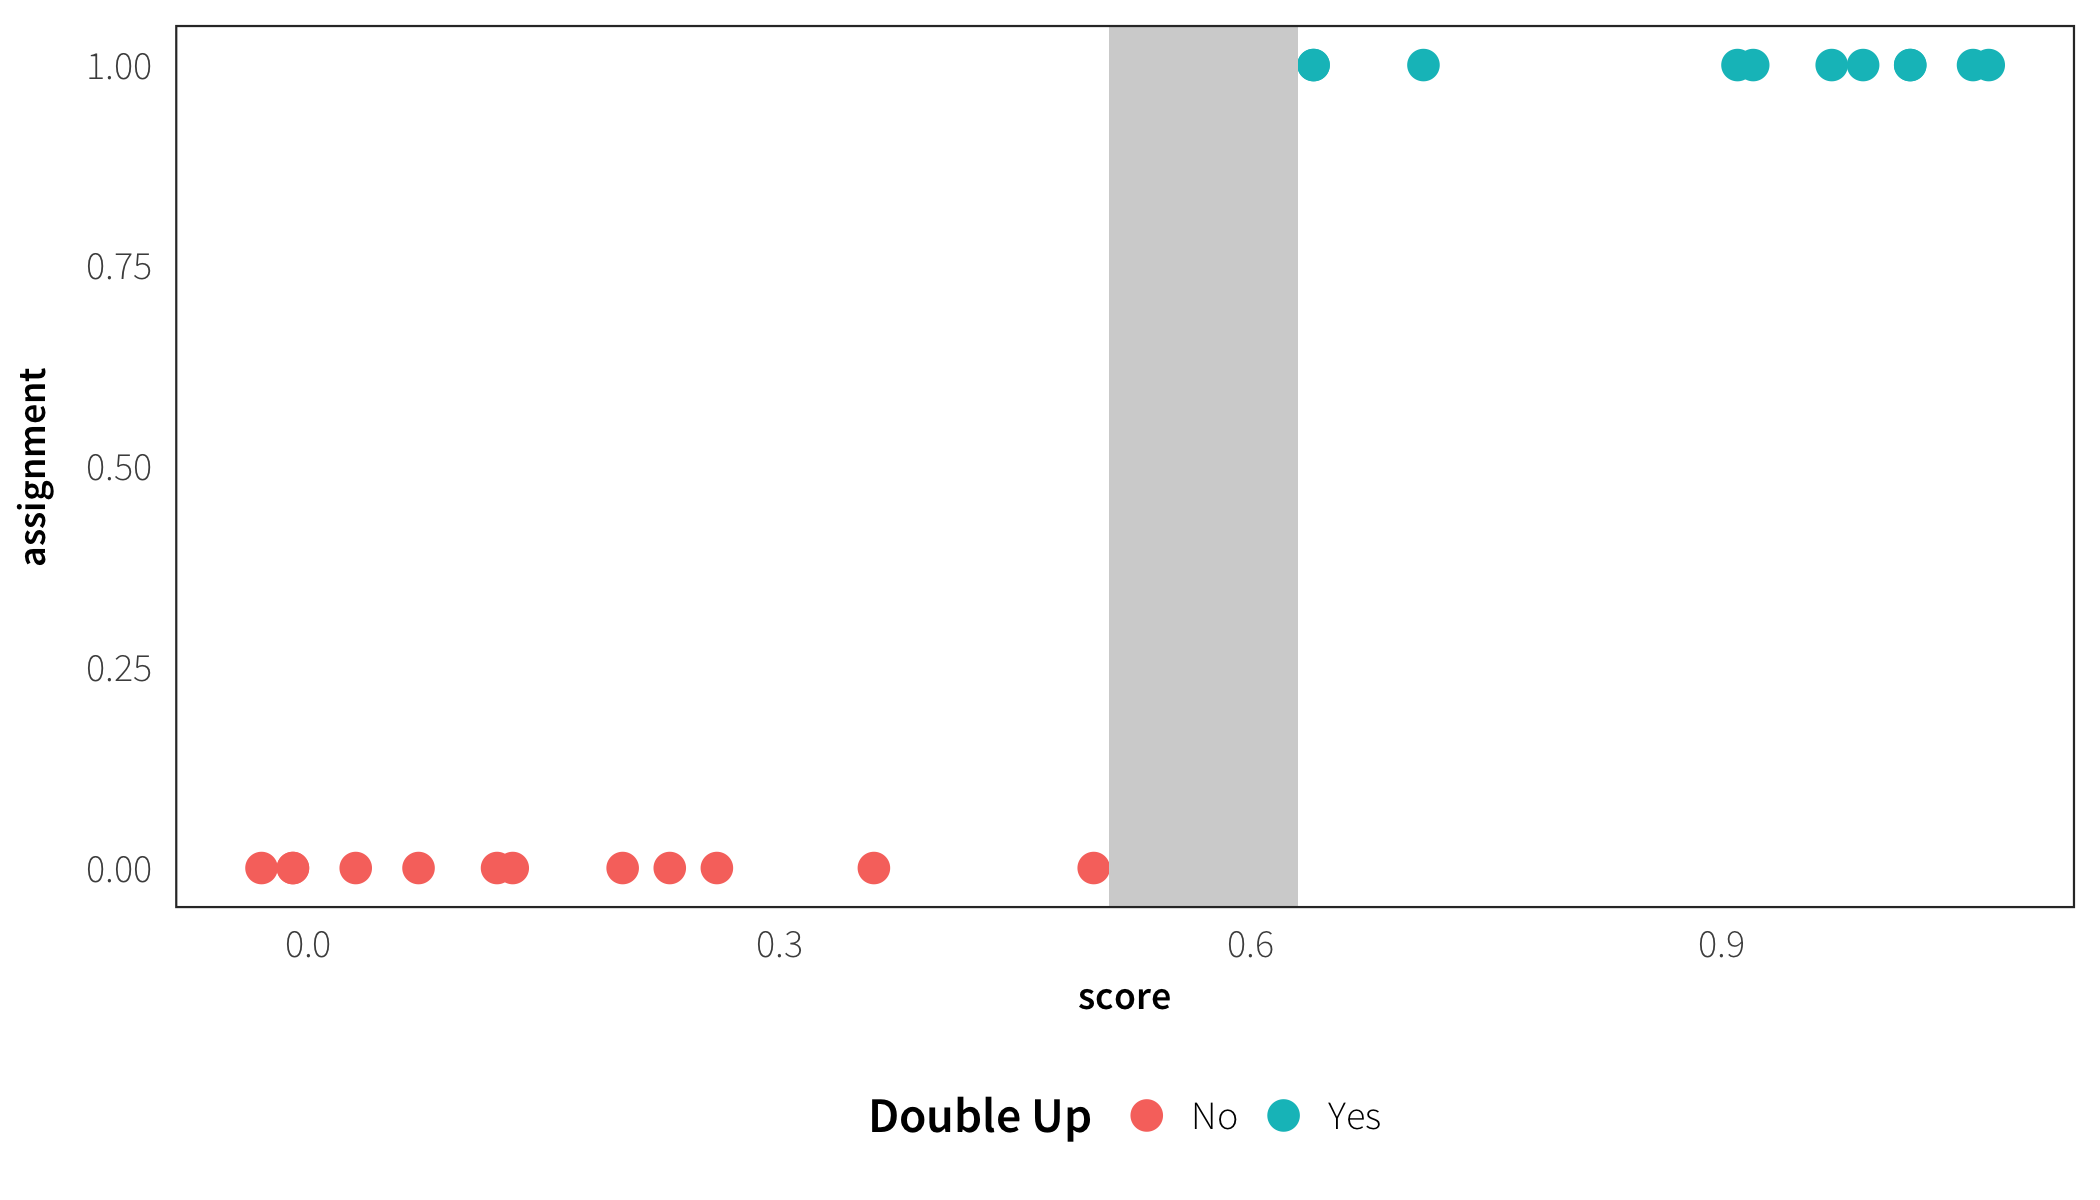
\includegraphics{noriega-prospectus_files/figure-latex/score-plot2-1.pdf}
\caption{\label{fig:score-plot2}Store Score vs Double Up Assignment with
Uncertainty Band (light gray)}
\end{figure}

I propose to estimate the RD design using various values of \(c\). The
perpetual gap means any model estimate to the left or right of some
\(c_0 \in (0.50, 0.64)\) will have to be extrapolated up to \(c_0\).

\textbf{Set-up}

The outcome of variable, as before, is \emph{the total daily amount of
dollars spent on fruits and vegetables per store transaction}. I decided
on using days as the unit of observation to increase the amount of data
for estimation. I expect there to be enough transactions per day for
this to be possible. The time frame will be August - December (months
\(8\) - \(12\)) of 2016, when the DUFB incentive is place. Only SNAP
transactions will be considered and transactions will be pooled. Given
that stores may vary in sales volume sold, I may divide by total SNAP
dollars spent and use proportions. In total, there will be \texttt{11}
treated (experimental) stores and \texttt{12} control stores.

Let \(y_{jt}\) represent the outcome variable where \(j=1,...,N\)
denotes stores across \(t=1,...,T\). Let \(c\) denote the cutoff;
\(s_{j}\) the score computed for store \(j\); and \(D_{j}\) the
assignment variable. Each draw (or row) of data for store \(j\) is a
vector \((y_{jt}, s_{j}, D_{j})\) corresponding to a single day.
\(\lambda_t\) are time effects and \(u_{jt}\) is an idiosyncratic store
level error term.

The RD model I propose follows the setup of \citet{lee_regression_2010}
(section 4.3):

\[y_{jt} = \alpha + \lambda_t + \rho D_{j} + \gamma (s_{j} - c) + \delta D_{j}(s_{j} - c) + u_{jt}\]

\textbf{Expected Results}

Plotting RD data and observing a visual gap is standard. The first thing
I would do is plot the outcome variable of interest---total daily
(fraction of) SNAP dollars spent on fruits and vegetables---against the
running variable \(s_j\). A total of \(N \times T\) (23 \(\times\) 153)
data points exists; each value of \(s_j,~j=1,...,23\) will contain
\(T=153\) points.

The graph produced will have more gaps compared to conventional RD
graphs. In more conventional RD graphs, each point represents a single
value for a single person (e.g.~score on an exam), producing more points
along the running variable axis. I do not have enough stores to produce
enough \(s_j\) values for this to be possible. Instead, this RD design
plots multiple points per stores, creating a distribution such that the
mean (or median) value (with some confidence interval) becomes the
fitted values of interest. Estimation wise, this distinction changes
little; \(E[y_{jt}|s_{j}, D_{j}]\) effectively fits a mean value to each
different store. But graphically, what matters in my RD is the overlap
between distributions before and after the cut-off point.

\chapter{The Durham Connects RCT and Applications for Social
Services}\label{chapter-2}

\section*{Motivation}\label{motivation-1}
\addcontentsline{toc}{section}{Motivation}

\textbf{Research Question}

\begin{quote}
Did assignment to the Durham Connects (DC) RCT impact a family's future
probability of applying for social services? That is, for families
assigned to DC during the trail period, I want to see if the
intervention (nurse home-visit) increased the probability of applying
for social services \emph{sooner} and/or overall.
\end{quote}

\textbf{Hypothesis}: I expect to observe a larger proportion of
families, randomly assigned to the Durham Connects program, requesting
social services. This would include social services like the
Supplemental Nutrition and Assistance Program (SNAP), Temporary
Assistance for Needy Families, Child Care Subsidies, and Medicaid.

My hypothesis is that the information and nurse contact provided to DC
families decreased the complexity of applying and navigating the social
safety net. As a result, I expected DC families will be observed
applying for social services sooner and/or more frequently, not because
they are, on average, in greater need of assistance, but because they
were better informed and more encouraged to seek out available
resources.

The RCT design of the Durham Connects program allows me to make certain
assumptions with reasonable confidence. Without these assumption, my
research question would be difficult to answer.

The first assumption is that random assignment resulted in balanced
groups. Eligibility for social services is a function of income and
demographics, and I'm assuming these are, on average, the same between
the treatment and control groups. I have no way to test balance along
income, but I can attempt to check balance along race/ethnicity using
first and last names.

The second assumption is a high compliance rate. I'm assuming that a
majority of families assigned to DC accept and commit to the nurse
home-visit. This assumption should be easy to verify. Compliance is
important because any effect the nurse home-visit may have on social
service application is going to be driven by the complying population.
The nurse is who assesses the mother and child's health and home
environment. These assessments, in turn, determine follow-up visits,
educational resources, recommendations to programs, and, if needed,
referrals---the mechanisms that I believe reduced learning and
administrative costs.

The last assumption, related to the first, is valid model
identification. Assignment to DC is random. By construction, it's
exogenous to observable and unobservable variables. It's also easy to
defend the idea that assignment to DC has a direct impact on
recommendations and referrals by nurse home-visitors. Assuming valid
model identification is reasonable given such a good instrument.

\section*{Introduction}\label{intro-2}
\addcontentsline{toc}{section}{Introduction}

Not all individuals that are eligible for social services apply to
receive them. The proportion of those eligible for a social service that
are actually receiving the service is known as the ``take-up'' rate.
Ideally, given complete information about eligibility and the existence
of social service programs---and zero costs in applying for, or
receiving, government assistance---the take-up rate would be 100\%. To
do otherwise would be to ``leave money on the table''---a violation of
neoclassical economic theory. In the United States and across the globe,
however, most social service programs never reach a full take-up rate.

Explanations for low take-up rates are numerous. Economists, for
example, developed models of social stigma to explain an individual's
decision for not applying for government assistance
\citep{moffitt_economic_1983}. ``Stigma'' broadly encompasses any cost
that reduces the total utility acquired from receiving government
assistance. Stigma and available benefits can vary across individuals.
Those with insufficient net benefits, after considering the cost of
stigma, would reasonably choose not to apply for government assistance.
That is, the take-up rates can fall below 100\% within any set of
eligible individuals when the cost of stigma outweighs those of the
benefit. We can extend the costs of stigma to include other standard
costs, like transaction costs or search costs.

Low take-up rates can also be explained by relaxing standard
neoclassical assumptions, like complete information. If one instead
assumes that most individuals have \emph{incomplete} information about
existing social services programs and corresponding eligibility
requirements, then lower take-up rates are unsurprising. Eligibility
requirements, for example, are dynamic. Families and individuals can
fall in or out of eligibility given a change in policy, leaving families
with an outdated understanding of requirements. For example, following
welfare reform in 1996, federal requirements shifted for programs like
Medicaid, Supplemental Security Income (SSI), and cash assistance
(renamed to Temporary Assistance for Needy Families or TANF). Welfare
reform also gave more power to states to determine eligibility
standards. Dissemination and implementation of these new eligibility
requirements was not instantaneous and the confusion lead to a reduction
in take-up rates for some programs \citep{stuber_stigma_2004}. Shifting
requirements aside, many families that are eligible for social service
programs can be misinformed or confused. It can be difficult to navigate
the application process when requesting government assistance.
Information about programs and their eligibility requirements is diffuse
and complicated. We do not expect everyone to fully grasp how to
complete their taxes without assistance or making errors. Likewise, we
should not expect families coping with poverty to be fully informed
about benefit levels or the application process of every existing social
service program.

Behavioral economics offers other compelling reasons for low take-up
rates. Status quo bias, for example, is a common task-completion
deterrent \citep{kahneman_anomalies:_1991}. Simple inertia means that
most people will procrastinate. This can keep any person from completing
things like applications, making doctors appointments, or even folding
laundry. Bounded rationality and the human tendency to use heuristics
for decision making also reduce take-up rates. Often, individuals
assume, based on some rule-of-thumb, that they must not be eligible. If
this assumption is never challenged, either by seeking out information
or having it provided, then they will never discover otherwise.
Time-inconsistent preferences also present a challenge for take-up
rates. Hyperbolic discounting implies that humans will favor putting off
any decision where gains are felt far in the future but losses are felt
almost immediately. In applying for government assistance, future
benefits are discounted heavily while the short-term cost of applying
are not \citep{currie_take-up_2006}.

A simpler explanation for low take-up rates is the existence intentional
bureaucracy. Governments purposefully make the application process
burdensome and confusing to deter applications. The take-up rate of
TANF, for example, has plummeted since the federal government overhauled
welfare in 1996 \citep{ribar_how_2014}. TANF gave enormous leeway to
states on how to distribute TANF dollars with little oversight. As a
result, over the last 20 years states have shifted away from using TANF
dollars for its intended purpose of providing cash assistance to needy
families.

On average, 26 percent of TANF dollars go towards provided basic cash
assistance \citep{schott_how_2015}. This drop in TANF take-up rates has
coincided with increasingly strict TANF eligibility requirements. This
is particularly true in state and local governments with a long history
of racial animus towards minorities and the ``undeserving'' poor, like
in the deep south \citep{keiser_race_2004}. North Carolina, for example,
added a drug testing requirement to its TANF program known as ``Work
First'' \citep{lynn_bonner_nc_2016}. These requirements tend to
disproportionately affect minority families because they are more likely
to be sanctioned by local caseworkers for failing to meet requirements
compared to white families \citep{monnat_color_2010}. This both increase
the cost of acquiring TANF benefits \emph{and} increases the chances of
losing access to an already difficult-to-acquire benefit. All in all,
take-up rates for some social service programs can be low because state
and local governments are actively increasing the costs for applying and
maintaining benefits.\footnote{It is important to note that there is
  also research showing application complexity always punishes the poor.
  When applying for federal student aid, which is open to all families,
  increased complexity burdens poor families the most. This further
  implies that the poor are also those most likely to benefit from
  targeting marketing and educational assistance. See
  \citet{dynarski_cost_2006} and \citet{bertrand_behavioral_2006} for
  more.}

Low take-up rates should concern policy makers. The positive impact many
government programs have on quality of life is well researched. For
example, passage of the Affordable Care Act gave states the option to
expand Medicaid coverage. This increased the pool of who was eligible
for Medicaid. For those previously without health insurance, Medicaid
coverage increased self-reported health status, lowered rates of
depression, and reduced financial strain and poverty
\citep{baicker_oregon_2013, sommers_mortality_2012, sommers_poverty-reducing_2013}.
Families that participate in the Supplemental Nutrition Assistance
Program (SNAP) increase the nutritional value of their diet and free up
cash for use on other priorities, like health care
\citep{bartfeld_snap_2015, sonik_massachusetts_2016, miller_using_2017}.
Increased use of the Earned Income Tax Credit (EITC) increases cash on
hand, improves educational outcomes for children, and improves labor
market out comes for adults
\citep{grogger_effects_2003, bhargava_why_2012, dahl_impact_2012}.
Lastly, eligible families that participate in the Special Supplemental
Nutrition Program for Woman, Infants, and Children (WIC) see improved
child health outcomes when compared to eligible non-participating
families \citep{bitler_does_2005}. Therefore, considering the positive
impact of most government assistance programs, it should be a priority
to champion any low-cost policy changes that increase take-up rates.

In the next section, I will introduce the Durham Connects (DC) program
and how I believe it may have helped increase requests for social
service programs. Note that increasing requests for social services is
not equivalent to increasing take-up. A request for service, however, is
a necessary first step for any eligible participant to receive benefits.
Increased requests, therefore, serve as a proxy for increased take-up
rates.

\subsection*{The Durham Connects Randomized Control
Trial}\label{the-durham-connects-randomized-control-trial}
\addcontentsline{toc}{subsection}{The Durham Connects Randomized Control
Trial}

The \href{https://www.durhamconnects.org/about/}{Durham Connects} (DC)
program is a postnatal nurse home-visiting program designed to be
universal, short-term, and less intensive than other nurse home-visiting
programs like Healthy Families America and Nurse-Family Partnership. The
DC program, in brief, aims to celebrate with new mothers, support and
connect then with community resources, and then follow-up if necessary.

Before expanding, a randomized control trial (RCT) of the DC program was
implemented from July 1, 2009 to December 31, 2010 to determine its
efficacy. The RCT included \texttt{4777} births from two Durham
hospitals. These two hospitals account for a vast majority of births in
Durham County. The randomization procedure assigned all babies born on
even days to the DC program. Babies born on odd days were assigned to
the control group, and were not invited to receive a DC home visit.

For those assigned to the treatment group, soon after birth a DC program
liaison at the hospital scheduled a home-visit by a registered nurse
with the infant's family. The initial home-visit was generally scheduled
about 3 weeks following the birth. During the initial home-visit, the
nurse assessed and rated 12 factor along 4 domains of family support:
health of the mother and child, the safety of the home environment,
planning care for the infant, and general wellbeing of the parent(s).
Each of the 12 factors received a rating between \texttt{1} and
\texttt{4} from the home-visiting Nurse. Each number represented varying
levels of need and risk:

\begin{itemize}
\tightlist
\item
  \texttt{1} - No risk/needs. General supportive guidance provided.
\item
  \texttt{2} - Low risk/needs. Concerns can be addressed by education
  and in-home demonstrations during visit.
\item
  \texttt{3} - Moderate or high risk/needs. Family are linked with
  community resources best suited to support risk areas.
\item
  \texttt{4} - Urgent needs. Immediate intervention required.
\end{itemize}

Follow-up visits were scheduled as necessary. Generally, the more
support a family needs, the more follow-up visits would occur.

Prior research has used the RCT to evaluate some aspects of DC. Notably,
\citet{dodge_implementation_2013} found that the DC nurse home-visiting
program reduced emergency medical care costs and increase health
outcomes for both mother and child. Furthermore, the DC program was
found to be cost-effective, saving an estimated 3 dollars in medical
costs for every dollar spent on implementation. In short, DC was
impressively successful at improving the physical health and mental
health of mother and child.

I'm interested in using the randomized assignment to measure what I
would consider a secondary effect of the nurse home-visiting program. An
essential part of the program was establishing a link between DC
families and Durham Social Services (DSS) to ``facilitate the \ldots{}
ease of access to and knowledge about eligible services''
\citep{odonnell_family_2015}. I hypothesize that by providing a trusted
contact (the nurse), educational resources, and a link to local social
services, a secondary effect of the DC program was that participants had
a higher application rate for social services than non-participants.

The nurse--patient relationship is key to the success of the DC program.
The days and weeks following a new birth are periods of high need for
both mother and child \citep{organization_who_2013, evans_cohort_2001}.
High need for postnatal/postpartum support means new mothers and
families are more willing to accept help when offered---especially from
nurses and nurse-centered programs. Patients, generally, view nurses
favorably, but interactions tend to be viewed more positively when they
occur outside the hospital/clinic environment
\citep{jansson_first-time_2002}. Likewise, perceptions about community
health programs tends to be more positive when they are known to be
organized and conducted by nurses \citep{kneipp_reasons_2009}. Nurses
that assist in home-visiting program for new mothers, in particular,
tend to be viewed very positively by their patients---as both a
professional expert and friend \citep{landy_mothers_2012}.

While initial DC home-visits may be brief in some cases (e.g.~rating is
\texttt{1}), new mothers requiring the most support and resources are
visited more than once. Nurses are most involved with families that
receive factors rated \texttt{3} or \texttt{4}. In these instances,
families are \emph{referred} to Durham Social Services for help. That
is, DSS is made aware that the family is in need of a specific type of
support and, with the help of the nurse, links up with the family
directly. This is distinct to families with factors of only \texttt{1}
and/or \texttt{2}. For these families, nurses only \emph{recommend}
community services and resources. The option to utilize the resources is
then left to the family.

In both cases, however, notice that the nurse is, in one way or another,
reducing the costs associated with applying for social services. At a
minimum, the nurse reduces the \emph{search} costs for families by
provided information for resources. At a maximum, the nurse connects
families with DSS directly to determine eligible services. In the latter
case, the nurse, in partnership with DSS, also lowers the
\emph{transaction cost} of applying.

I should pause to specify what it meant for a family to be ``connected
with DSS''. It is my understanding that this means a family was put in
contact with, or place ``on the radar'' of, a specific DSS worker
assigned to assist DC families (name omitted). The degree, and success,
to which this worker was involved in assisting families apply for
services would have had a impact on application rates. I have yet to
interview this person, but I plan on doing so.

\newpage

\section*{Concept in a Plot}\label{concept-in-a-plot-1}
\addcontentsline{toc}{section}{Concept in a Plot}

\begin{figure}
\centering
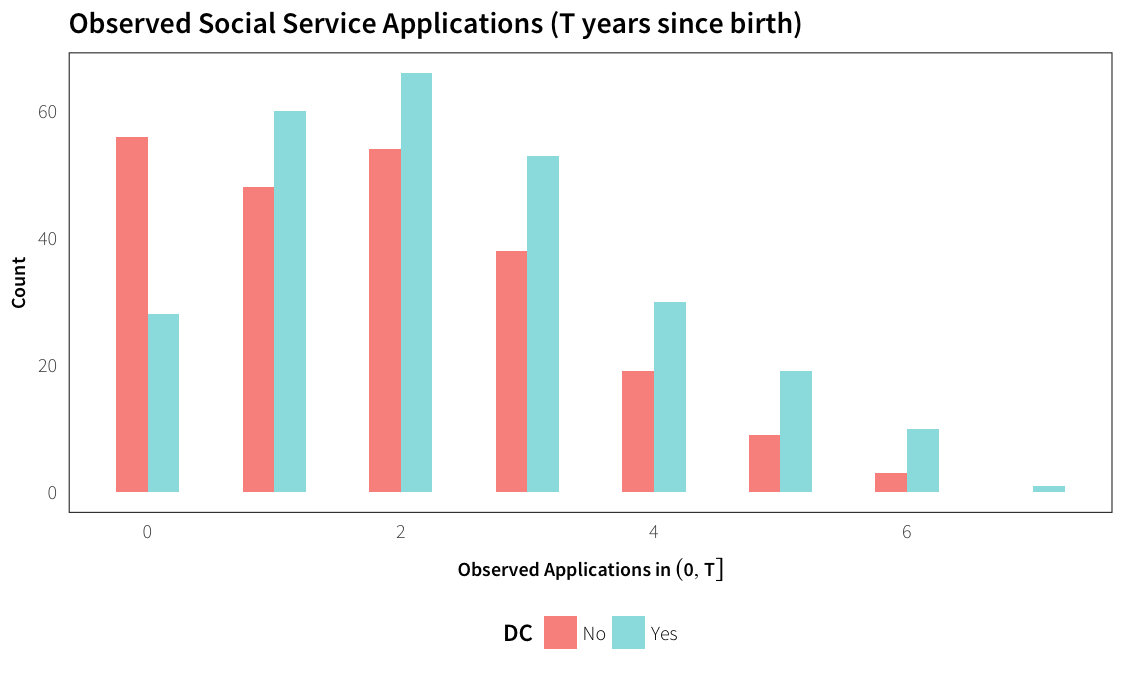
\includegraphics{noriega-prospectus_files/figure-latex/plot-dc-1.pdf}
\caption{\label{fig:plot-dc}Example of Hypothetical Result (Fake Data)}
\end{figure}

Figure \ref{fig:plot-dc} represents what I would ideally observe in the
data should my hypothesis prove correct. Unit of analysis is aggregated
counts of observed applications (requests) per person between time
\texttt{0} and \texttt{T} (\texttt{T} is some fixed unit of time,
perhaps 1 or 2 years). Time \texttt{0} is the date of birth for the baby
that is (or is not) assigned to the Durham Connects RCT.

The histogram of green bars represents counts for parents that were
randomly assigned to DC. Red bars are those assigned to the control.
Should my hypothesis prove correct, then I would see, in aggregate per
person, more requests for services from families assigned to DC.

Note that these distributional comparisons are not the best way to test
any hypothesis with what is event data. I also do not expect to see so
many applications per person. In fact, what I care about is if DC
increase the likelihood of applying at all. But that graph looks far
less interesting.

\newpage

\section*{Data}\label{data-2}
\addcontentsline{toc}{section}{Data}

This paper will depend on two sources of data. The first data source is
Durham Social Services (DSS). DSS has provided administrative records to
determine what services where applied for and by whom. The second data
source is the Center for Child and Family Health at Duke University
(CCFH). CCFH has already collected the short-form birth records of all
children born during the RCT. While these data are public record, access
to CCFH's data would drastically reduces the burden of acquiring these
data.

For example, were I not to use CCFH's data, I would have to requests the
short-form birth records, wait to receive them, and then manually input
the records data into a spreadsheet (the birth certificate come as
digital copies of the paper certificate). That would take an incredibly
long time. Furthermore, CCFH was able to verify if the short-form birth
records received contained any errors. This is because they have access
to their own records collected during the RCT. CCFH found and corrected
six errors. I would not be able to do the same corrections on my own.

\subsection*{Administrative Records}\label{administrative-records}
\addcontentsline{toc}{subsection}{Administrative Records}

Durham Social Services provided the Durham Children's Data Center (DCDC)
with access to their administrative records. The pertinent data within
the collection provided is known as the \emph{Scheduler} data. This is a
database that logs all request for social services assistance from the
DSS.

I do not yet have explicit permission to write about what is in these
data. That said, I do not think I'm revealing anything obvious by noting
that the \emph{Scheduler} data contains name, age, service requested,
and date of request. These 4 variable are sufficient to explain my
methodological approach. I have access to multiple years of data but
still need to verify if I have all that is available.

\subsection*{Short-form Birth Certificate
Data}\label{short-form-birth-certificate-data}
\addcontentsline{toc}{subsection}{Short-form Birth Certificate Data}

Short-form birth certificates are public record. It is possible, for
example, to request birth records directly from the
\href{http://vitalrecords.nc.gov/order.htm}{North Carolina Department of
Health and Human services}. Collecting all recorded births in Durham
County from the 2 largest hospitals would take a considerable amount of
time. Fortunately, the CCFH already collected and corrected the
short-form birth certificate data.

Short-form birth certificate includes sufficient information to identify
which families were randomly assigned to Durham Connects. It also
provides enough information to identify parents should they appear in
other administrative records that contain name and date-of-birth.
Specifically, the child's date-of-birth, the child's name, the mother's
maiden name, and the father's name (if present).

These four pieces of information are enough to search and tag when the
parents of a child born during the DC RCT applied for services. The
child's date of birth is all that is required to determine assignment
status.

\subsection*{Matching Strategy}\label{matching-strategy}
\addcontentsline{toc}{subsection}{Matching Strategy}

An important step will be to link the two datasets. This will likely be
done by matching on the names of the parents and dates of birth. Fuzzy
matching procedures for character strings exists in \texttt{R} and
\texttt{Stata}. I do not think this will too difficult or
computationally intensive as the set of names that need to be searched
for is quite small (about \texttt{5000}).

\subsection*{IRB and Permissions}\label{irb-and-permissions}
\addcontentsline{toc}{subsection}{IRB and Permissions}

Currently, I am in the process of submitting an IRB request to access
the CCFH's database contain the digitized and curated public short-form
birth records.

I am also waiting to hear if I have permission from the director of
Durham Social Services to link these two data sets. I have no reason to
believe the director will not approve. It is just a matter of having an
opportunity to sit down and explain the idea and what it entails. The
meeting is anticipated to occur in late March.

\section*{Methods}\label{methods-2}
\addcontentsline{toc}{section}{Methods}

Methods for this paper are greatly simplified by the fact that
assignment to Durham Connects was \emph{random}. This provides an
instrument where, by design, the exclusion restriction is true (always
exogenous) given almost any outcome variable of interest. For this
study, I am interested in Durham Social Services \emph{applications},
which will serve as a proxy for take-up rate. Requesting (applying for)
government assistance does not guarantee receipt of benefits. But
applying is a necessary step for any eligible individual/family.

\subsection*{A Simple Model of Social Service
Demand}\label{a-simple-model-of-social-service-demand}
\addcontentsline{toc}{subsection}{A Simple Model of Social Service
Demand}

A simple economic model helps illustrate how I believe the Durham
Connects program may help increase take-up.

Assume all individuals value government benefits and incur the same
costs when applying for benefits. Individuals, however, have different
characteristics. These characteristics determine both eligibility and
size of benefits. Let's also assume complete information, rationality,
and that errors when applying are non-existent.

Individual \(i\) with characteristics vector \(\bm{x_i}\) will apply for
government assistance only if the \emph{net benefit} amount is greater
than zero. That is,

\[
r_i  = \left \{
  \begin{array}{c}
    1 \text{ if } NB(\bm{x_i}, c) > 0 \\
    0 \text{ if } NB(\bm{x_i}, c) \le 0
  \end{array} \right.
\]

\[
  NB(\bm{x_i}) = B(\bm{x_i}) - c
\]

where \(r_i\) is the decision to apply for benefits; \(NB(\bm{x_i}, c)\)
is the net benefit; \(B(\bm{x_i})\) is the benefit amount as a function
of individual characteristics, \(\bm{x_i}\); and \(c\) is the cost of
applying. Eligible individuals have a value \(B_i > 0\). Note that for
convenience, \(B_i \equiv B(\bm{x_i})\) and
\(NB(\bm{x_i}, c) \equiv NB_i\)

My hypothesis is that the Durham Connects program reduces the cost of
applying. In this simple model, assume that the DC program drops the
cost of applying down to some \(\tilde c < c\). Let \(d_i = 1\)
represent assignment to DC. Before assignment, each individual is
eligible for net benefits

\[NB_i|_{d_i=1} = NB_{i1} = B_i - \tilde c\]
\[NB_i|_{d_i=0} = NB_{i0} = B_i - c\]

such that \(NB_{i1} > NB_{i0}\) for all individuals. This implies,

\[P(r_i = 1|d_i = 1) \ge P(r_i=1|d_i = 0)\]

In words, if assignment to DC reduces the costs of applying, then the
probability of applying for all individuals must either increase or stay
the same. Under this framework, this would imply that there must exists
a population of eligible individuals (\(B_i > 0\)) such that
\(NB_{i1} > 0\) but \(NB_{i0} < 0\). All other individuals are either
ineligible (\(B_i \le 0\)) or their application decision remain
unchanged after assignment (\(B_i > 0\) but \(NB_{i1} > NB_{i0} > 0\) or
\(NB_{i0} < NB_{i1} \le 0\)).

In reality, the cost of applying is also a function of (both observed
and unobserved) individual characteristics. But the model, even with
simple costs, still helps to illustrate why I believe the DC program may
lead to higher observed counts within the treated group.

\subsection*{Analytical Framework}\label{analytical-framework}
\addcontentsline{toc}{subsection}{Analytical Framework}

I plan to use the local average treatment effects (LATE) framework to
measure changes in the timing and volume of applications to Durham
Social Services \citep{angrist_mostly_2008}. I can be reasonably
confident that, whatever the measured difference between the two
subpopulations, it was driven solely by \emph{compliers}.

In this context, \emph{compliers} are assigned to the treatment (Durham
Connects) and do not back out from the nurse home-visit.
\emph{Non-compliers} are families with a child born on an even day that
opted out of DC or a child born on an odd day that found a way into DC.
\emph{Never-takers} are families that would never accept a home-visit
and \emph{always-takers} are families that found a way to participate in
Durham Connects.

I expect never-takers to have existed but do not know if there were any
always-takers. Until I find evidence otherwise, I will assume no
always-takers. Likewise, I need check and see if any families with
children born on odds days found a way into DC. If this happened, I'm
assuming records exists and I can remove them from the analysis. I will
also need to check how many families with children born on even days
opted out of DC. I believe this did occur but I don't know the opt-out
rate. However, I'm sure CCFH has this data and will provide it once the
IRB is approved.

If I observe any differences in the \emph{timing} or \emph{volume} of
applications between the treatment and control group, I can be
reasonably confident that the effect will come from the complying
population. This is because only the complying population should have
received a nurse home-visitor. Any observed differences would then be a
function of the information, recommendations, and/or referrals generated
by the nurse assessments. If the treated group is found to have earlier
application times or higher application rates, then I would expect
recommendation and referrals helped reduce the cost of applying. If no
differences are found, then the assessments either generated few
recommendations and referrals or the recommendations and referrals were
ineffective. That is, referrals or recommendations provided no new
information, opportunities, or reduced costs to eligible families.

I want to elaborate on what I mean by the \emph{timing} and
\emph{volume} of applications. That an eligible family choose to apply
for a service would affected that family's application \emph{volume}.
But also important was the \emph{timing} of the application. That a
family applied earlier than they would have otherwise is important. As
mentioned, hyperbolic discounting and status quo bias push humans to
procrastinate. I could count the number of applications submitted within
a fixed window (say, 2 years) between the two groups and find no
differences. Lost in this comparison, however, would be the
\emph{timing} of the applications. That is, if the treated group
happened to submit the same amount of applications as the control group,
but did so \emph{sooner} than the control, that difference would be
missed.

To this end, I propose using two analytical approaches. The first is a
simple Probit model. For the outcome variable, I determine which
families with children born during the RCT were observed during some
fixed period of time. I will then pool all families and regress whether
or not they were observed on a vector of observed characteristics,
eligibility, assignment group, and other variables, like distance from
the DSS office.

This first approach is inelegant and ignores some very important aspects
of the application process. For example, this totally ignores that
eligibility for social services is dynamic. For example, families
receive SNAP benefits during a fixed number of months known as a
``certification period''. But families can have discontinuous
certification periods if they lose eligibility or fail to renew. This
model, however, is useful if I make the assumption that dynamic movement
in and out of certification periods is similar between the two groups.
That is, I'm assuming the two groups are balance in both observable and
unobservable character, such as eligibility, even over time.

The second model will be a Cox proportional hazard (Cox PH) models for
recurrent events. These event models explicitly account for time and
counts. I must admit, though, that these recurrent event models are new
to me but I understand the basics enough to get how to structure the
data. (I can certainly see that there is a relationship between Poisson
regression and any hazard model.) I'm still deciding what type of Cox PH
model suits this study (see Chapters 7 and 8 of
\citet{aalen_survival_2008}).

\subsection*{Poisson Regression Model with Pooled
Data}\label{poisson-regression-model-with-pooled-data}
\addcontentsline{toc}{subsection}{Poisson Regression Model with Pooled
Data}

Assume I've collected data for some fixed interval of time \(T\) and
know the complete population of RCT individuals, \(N\). Any individual
observed applying for assistance is tagged \(y_i=1\). Those never
observed are tagged \(y_i=0\). I'm assuming that the treated and control
groups are balanced along both observed and unobserved characteristics.
The probit model is as follows:

\[
w^* = \bm{x'\beta}  + \delta D + u, \quad u \sim N(0, \sigma^2)
\]

\[
P(y=1|\bm{x}, D) = \Phi \left (\frac{\bm{x'\beta}  + \delta D}{\sigma} \right ), \quad
y = \left \{
  \begin{array}{cc}
    1 & \text{ if } w^* > 0 \\
    0 & \text{ otherwise}
  \end{array}
  \right .
\]

\[
\star ~ E[u|D] = 0 ~ \star
\]

The emphasis on \(E[u|D] = 0\) is to reiterate that assignment, \(D\),
was random, and is therefore \emph{exogenous}. What I care to find out
is the difference in probability of observing \emph{any} social service
application given \(D\). Furthermore, my hypothesis is that it leads to
an \emph{increase}, such that

\[
\begin{aligned}
  E[y|\bm{x}, D=1] - [y|\bm{x}, D=0] &> 0 \\
  \\
  \Rightarrow E \left [
        \Phi \left (\frac{\bm{x'\beta}  + \delta}{\sigma} \right )
      -
        \Phi \left (\frac{\bm{x'\beta}}{\sigma} \right )
     \right ]  &> 0
\end{aligned}
\]

Of course, since \(E[u|D] = 0\), the average treatment effect (ATE) is
sufficient (and without bias)

\subsection*{Stratified Cox Proportional Hazard
Model}\label{stratified-cox-proportional-hazard-model}
\addcontentsline{toc}{subsection}{Stratified Cox Proportional Hazard
Model}

TDB.

\chapter{The SNAP Benefit Cycle and the Demand for Emergency
Assistance}\label{chapter-3}

\section*{Motivation}\label{motivation-2}
\addcontentsline{toc}{section}{Motivation}

\textbf{Research Question}

\begin{quote}
Do requests for local-government emergency assistance increase towards
the end of a household's SNAP benefit cycle?
\end{quote}

\textbf{Hypothesis}: I expect, on average, an increase in demand for
emergency assistance towards the last 2 weeks of the month following
SNAP benefit transfers. That is, I expect to reject the null hypothesis
that request for formal assistance from SNAP households are randomly
distributed between transfer dates.

Formal assistance refers to any assistance---cash, goods---from a
government program, non-profit, or charity. In this paper, however, I
focus on \emph{emergency} formal assistance, where households apply for
one-time (nonrecurring) assistance. I also include an analysis of
aggregated food pantry data. This type of assistance can be recurring
but when and how it is utilized by households is also enlightening.

I plan to answer the question above in two ways. The first exploits the
random nature of North Carolina's SNAP transfer schedule. Households are
assigned a monthly transfer date based on the last digit of the head of
household's social security number. Using administrative records, I can
determine a households transfer date then check to see if, and when, any
household member applied for emergency assistance. I can then build a
discrete-time hazard model for each individual where the start time is a
household's transfer date and the event of interest is date of
application for emergency assistance.

The second approach uses food pantry data. These data cannot capture
individual level variation in SNAP transfer dates. It can only capture
aggregate trends observed within normal monthly calendar cycles.
However, I anticipate that demand for food pantry assistance will
increase, in aggregate, during the 4th week of every calendar month,
through the 1st. SNAP benefits are transferred from the 1st through 3rd
week of each month. Most households will have had access to SNAP
benefits for at least 2 weeks by the 4th week of each month. If most
SNAP household consume their SNAP benefits quickly, then overlapping
demand for additional food assistance will be highest during the 4th
week through part of the 1st.

\section*{Introduction}\label{introduction}
\addcontentsline{toc}{section}{Introduction}

Cash assistance to needy families fell dramatically after 1996---the
year welfare reform replaced Aid to Families with Dependent Children
(AFDC) with Temporary Assistance for Needy Families (TANF). TANF
profoundly changed how states prioritize and spend government welfare
dollars. The result has been a gutting of traditional cash assistance
programs over the last 20 years \citep{cbpp_chart_2016}. Cash assistance
used to account for 70\% of AFDC spending \citep{ziliak_temporary_2015}.
Under TANF, cash assistance has dropped to a national average of 26\%,
with ten states spending below 10\% \citep{schott_how_2015}.

Decreased access to cash assistance corresponded with increased demand
for in-kind ``cash-like'' assistance---most notably the Supplemental
Nutrition Assistance Program (SNAP)
\citep{us_department_of_health_and_human_services_welfare_2015}. SNAP is
the most popular cash-like assistance available to families coping with
poverty. At 45.8 million participants in FY2015, is also the largest
food assistance program in the US \citep{usda_fns_supplemental_2016}.
Millions of families not only depend on SNAP to provide sustained,
predictable access to food, but also as a cash-like income supplement.
But SNAP benefits are not cash; they cannot pay the rent or the bills.
And when economic instability forces families to make tough decisions,
it is a lack of cash that prompts families to search for help from
formal and informal networks of support.

SNAP benefits should act as a buffer, alleviating strained food budgets
and allowing families to shift cash towards other priorities, like rent,
utilities, and health care \citep{hoynes_snap_2015}. Theory, however,
assumes SNAP benefits are treated like cash; that an increase in SNAP
benefits should induce similar spending behavior as an equivalent
increase in cash. Or, in economic terms, that the marginal propensity to
spend SNAP benefits on food should equal the marginal propensity to
spend cash on food. This assumption is false; SNAP benefits are not
treated like cash. For example, when the 2009 American Recovery and
Reinvestment Act temporary increased SNAP benefits by an average of
\(13.6\%\), for every \(1\$\) dollar of SNAP benefits, \(48\) cents were
spent on food, compared to only \(5\) cents when given a dollar in cash
\citep{beatty_expenditure_2015}.

SNAP benefits are also inadequate. They fail to cover monthly food
expenditures for the majority of cash-strapped families---even when
families maximize every dollar by consuming cheaper, less healthful
foods \citep{wiig_art_2009}. This is not to say SNAP benefits don't
help. On the contrary, they are incredibly important. Many families
depend on SNAP. It can account for a majority of food expenditure. Some
families even schedule their lives and budget priorities around the
timing of their SNAP benefits \citep{edin_snap_2013}.

The inadequacy of SNAP benefits to carry families through the end of the
month, coupled with hyperbolic discounting, produces what is known as
the ``SNAP benefit cycle'' \citep{smith_effects_2016}. This negative
cycle is characterized by high spending within the first 3 days of
receiving SNAP benefits, followed by a sharp decline
\citep{goldin_is_2016}. In the days leading up to the next scheduled
monthly transfer, families often have no benefits left to spend on food
\citep{wilde_monthly_2000, shapiro_is_2005}. Low on cash and benefits,
families often sustain themselves by tighten their belts and consuming
less nutritious foods \citep{todd_revisiting_2015}. The cycle then
repeats.

The SNAP benefit cycle makes families vulnerable to unexpected negative
income shocks. When cash is limited, unexpected expenses can be
devastating. Health emergencies or job loss can strain cash supplies and
leave families homeless or hungry \citep{curtis_life_2013}. For families
coping with poverty, informal safety nets (e.g.~family, friends) tend to
be the first line of defense when cash needs are high and formal safety
nets like SNAP fall short \citep{schenck-fontaine_use_2016}. However,
informal safety nets are not always available. Family and friends for
those coping with poverty often struggle with similar levels of economic
insecurity. Limited access to cash means families on the most extreme
margins will turn to other forms of support, like food banks/pantries or
emergency social services for assistance.

Some formal services exists that can provide families with emergency
cash to pay for necessities like rent, electricity, and food. Food
banks/pantries are an example of formal service that can, for some
families, be considered emergency assistance. Emergency cash assistance
also exists to help with rent and utilities but access can be quite
restricted. Durham County Social Services, for example, provides
emergency TANF assistance, which is limited to a \$400 dollars per 365
days \citep{durham_county_department_of_social_services_directory_2016}.
Emergency food cards also exists, but SNAP recipients are
ineligible.\footnote{One of the conditions to receiving a food card is
  that households must sign up for SNAP.}

In this paper, I investigate how the SNAP benefit cycle affects demand
for emergency assistance from formal support networks. I hypothesize
that demand for emergency assistance increases towards the end of the
benefit cycle. I test my hypothesis by checking household demand for
emergency assistance and aggregate demand from food banks/pantries in
Durham County, North Carolina.

\section*{Data}\label{data-3}
\addcontentsline{toc}{section}{Data}

The main data for this proposed paper comes from Durham Social Services
(DSS) in North Carolina. Of the datasets provided by DSS, two pertain to
this paper. The first is the SNAP (or FNS) data. The second is request
for emergency assistance, known as the Community Access Database (CADB).

At the moment, I do not have permission to describe either data set in
detail. I also do not have permission to link these two datasets
together, despite being from the same source. I am waiting to receive
approval from the Director of DSS. I expect his support but have been
told not to show any data details or results.

The other data I plan to use comes from Urban Ministries of Durham. It
is their database of food pantry donations distributed per day. I
hypothesize that aggregate demand for food assistance is highest during
the 3rd and 4th weeks of any given calendar month. The second half of
every month is when the largest fraction of SNAP families would be out,
or running low, on benefits. I must emphasize that I do not expect the
increase to be dramatic. But I do expect to see a cyclical pattern where
the peak occurs near week 4.

\subsection*{Durham Social Services
Data}\label{durham-social-services-data}
\addcontentsline{toc}{subsection}{Durham Social Services Data}

\textbf{SNAP/FNS Data}

Without going into too much detail, the important thing to note about
these data is that they contain names of the household head and
dependents, a case numbers to link with other datasets, benefit amounts,
and the SNAP certification period in month. The current SNAP data is
also incomplete. It is missing many years of data and doesn't contain a
benefit transfer date. I'm working with DSS to fix each of these
problems.

From these data, what I care about most is names, case number, and the
SNAP transfer date, and the certificate periods. The case number is what
should link the SNAP data to the CADB data. Just in case, I can attempt
to fuzzy match by name. I can determine start times for any event study
using the benefit transfer data and the certificate period. The
certificate period helps determine if and when a household---that does
not renew---stops receiving benefits.

The transfer date variable is incredibly important. In the state of
North Carolina, transfer dates are determined by the last digit of
people's social security numbers. Social security numbers are mapped to
every odd day from the 3rd to the 21st of every month. Those ending in
\texttt{0} are mapped to the 3rd, \texttt{1} to the 5th, and so forth,
with \texttt{9} mapping to the 21st. Those without social security
numbers are mapped to the 3rd, creating a slight bump in probability to
an otherwise uniform distribution. This implies that transfer dates are
assigned essentially at random.

This randomness is essential towards identifying if events are impacted
by the SNAP benefit cycle. If, for example, the transfer date occurred
during the 1st of the month for all SNAP participants, then many other
calendar-month events---like rent payments, utility payments, or payment
schedules---become endogenous to the SNAP benefit cycle.

\textbf{CADB}

These data contain all requests made for emergency financial assistance.
For this paper, what matters is the applicants case number, name, date
of application, and type of assistance requested. As before, the case
number and name are to help link between CADB and SNAP. The date of
application and assistance type requested is the ``event'' of interest.

\textbf{Approach}

The first step is to identify overlapping years between the two
databases, SNAP and CADB. Once determined, the population of interest
will be sourced from the SNAP dataset. I will then search and tag any
names found in the CADB that overlap.

Next, I would need to determine continuity of SNAP benefits. This should
not be difficult given that the SNAP data has a certification variable.
This variable lists the months for which the household is to receive
SNAP benefits.

Once benefit continuity has been determined, I can then structure the
data for a hazard model. The specifics of the hazard model are to be
determined.

\subsection*{Food Pantry Data}\label{food-pantry-data}
\addcontentsline{toc}{subsection}{Food Pantry Data}

I recently received these data and have no yet taken a look at the
contents. It is a Microsoft Access Database file with, I expect, 2 or 3
years of daily data. I have, however, seen a printout for these data
from July 2016. The pattern, given the printout, seems to support my
hypothesis above---donations are highest towards the end of the month.

One thing to keep in mind is that demand for food can be higher than
what is actually distributed. UMD doesn't record who comes in requesting
food from the food pantry. Furthermore, donations are capped at 26
families per day. Families are then turned away once the cap is hit.
This means that more families could come in asking for food during
distribution hours (9 am to 11 am, Monday through Friday), but such
demands go unrecorded.

I should also note that these data are maintained by a single person at
UMD. The data is entered, however, by a different person---a volunteer.
This volunteer comes in every Tuesday and Thursday morning to manually
input the data. There is likely a bit of human error, but as long as a
general trend is noticeable, then it should be better than nothing.

I'm not sure if there is sufficient data here to run a regression that
wouldn't be bested by simply plotting the data. The food pantry data is
therefore excluded from my methods section.

\newpage

\section*{Concept in a Plot}\label{concept-in-a-plot-2}
\addcontentsline{toc}{section}{Concept in a Plot}

\begin{figure}
\centering
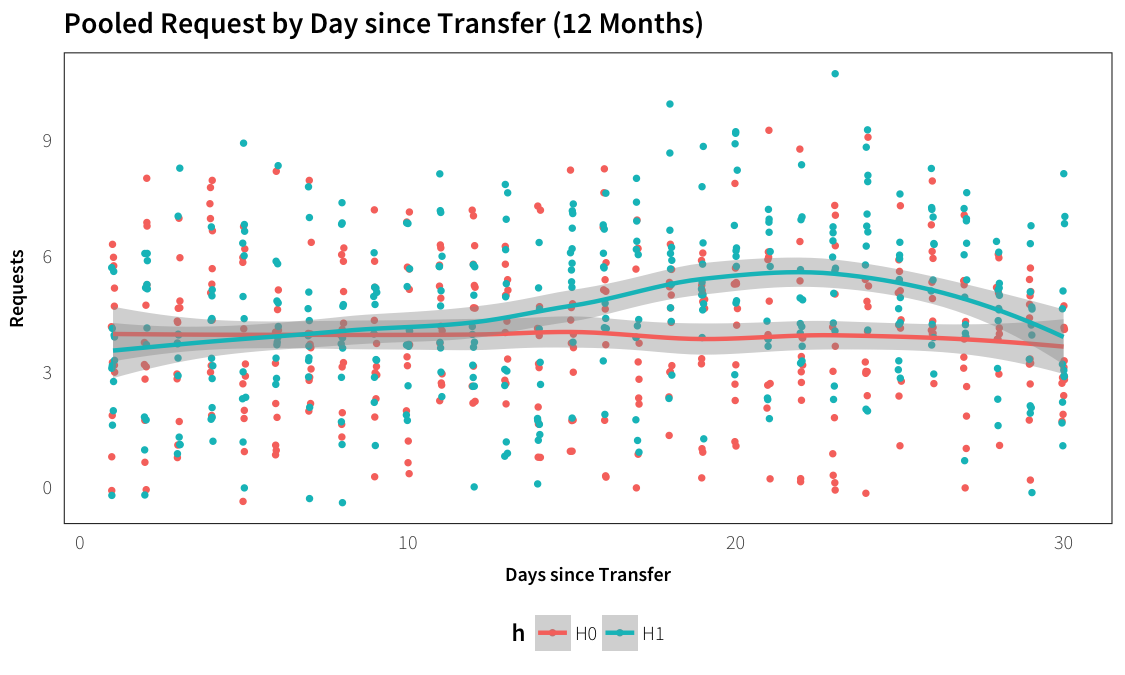
\includegraphics{noriega-prospectus_files/figure-latex/plot-cycle-1.pdf}
\caption{\label{fig:plot-cycle}Pooled Monthly Request for Emergency Services
by Day since Transfer using Fake Data}
\end{figure}

Here, \texttt{t=0} lines up with the SNAP transfer date for each
household. The green line in Figure \ref{fig:plot-cycle} represents what
I would ideally expect to find when exploring the administrative data.
That is, were I to count 12 months of request for emergency services by
day-since-transfer, I would expect the counts to be higher in the 3rd
and 4th week since transfer. The red line represents the null hypothesis
that the SNAP benefit cycle has no impact on demands for cash.

I suspect, however, that requests for emergency cash assistance will be
infrequent. I also suspect seasonality will have an important impact on
requests. For example, emergency assistance for utilities will likely
increase during winter months. All that is to say, my actual analysis of
the data will be different. Please see the
\protect\hyperlink{methods-3}{Methods} section for details.

\newpage

\hypertarget{methods-3}{\section*{Methods}\label{methods-3}}
\addcontentsline{toc}{section}{Methods}

I propose using a \emph{proportional frailty model} for recurrent events
(see Chapter 7; \citet{aalen_survival_2008}).\footnote{``Frailty'' is a
  fancy event history analysis word for unobserved heterogeneity aka
  endogeneity.} Is this the best model? I do not know. But more basic
models I've research assume that events of interest occur only once
\citep{singer_applied_2003}. I believe it probable that my event of
interest---an application for emergency benefits---will occur more than
once for some household heads.

I have a lot to learn about survival analysis. I would love to write up
a model for this draft, but I would be pretending to understand
something I've spent too little time thinking about.

I look forward to learning about how these methods. Until then, this
section will remain regrettably sparse.

\chapter{Healthy Food Experiments (BECR
Project)}\label{healthy-food-experiments-becr-project}

I'm working with a BECR Center team that is piloting a few random
experiments. The aim is to nudge people towards purchasing healthier
snacks. They are working in partnership with
\href{http://familyfareconveniencestores.com}{Family Fare Convenience
Stores} to run the experiments and collect the data.

In exchange for a co-authorship, I am helping will all things data.

I'm listing this to point out that \textbf{I have a back up paper}.

\bibliography{bib/book.bib}

\backmatter
\printindex

\end{document}
